% ============================================================
% 等离子体物理自学教材
% ============================================================
\documentclass[12pt,a4paper,openany,oneside]{book}
\usepackage[UTF8]{ctex}
\usepackage{geometry}
\geometry{left=2.5cm,right=3.5cm,top=2.5cm,bottom=2.5cm}
\setlength{\headheight}{15pt}
\usepackage{amsmath,amssymb,amsthm}
\usepackage{mathtools}
\usepackage{bm}
\usepackage{esint}
\usepackage{siunitx}
\usepackage{tikz,pgfplots}
\pgfplotsset{compat=1.18}
\usetikzlibrary{arrows.meta,decorations.pathmorphing,patterns,calc,positioning,shapes}
\usepackage{xcolor}
\usepackage{graphicx}
\usepackage{enumitem}
\usepackage{fancyhdr}
\usepackage{titlesec}
\usepackage{tcolorbox}
\tcbuselibrary{theorems,skins,breakable}
\usepackage{booktabs}
\usepackage{array}
\usepackage{caption}
\usepackage{subcaption}
\usepackage{hyperref}
\usepackage{cleveref}
\usepackage{braket}
\usepackage{float}
\usepackage{multirow}
\usepackage{marginnote}
\usepackage{epigraph}
\usepackage{makeidx}
\makeindex
\setlength{\marginparwidth}{1.2cm}
\setlength{\marginparsep}{0.4cm}
\pagestyle{fancy}
\fancyhf{}
\fancyhead[L]{\nouppercase{\leftmark}}
\fancyhead[R]{\thepage}
\renewcommand{\headrulewidth}{0.4pt}
\titleformat{\chapter}[display]
  {\normalfont\huge\bfseries}{\chaptertitlename\ \thechapter}{20pt}{\Huge}
\titleformat{\section}{\normalfont\Large\bfseries}{\thesection}{1em}{}
\titleformat{\subsection}{\normalfont\large\bfseries}{\thesubsection}{1em}{}
\definecolor{thmblue}{RGB}{41, 98, 255}
\definecolor{defgreen}{RGB}{46, 125, 50}
\definecolor{cororange}{RGB}{230, 81, 0}
\definecolor{exampurple}{RGB}{106, 27, 154}
\definecolor{insightred}{RGB}{183, 28, 28}
\definecolor{warnyellow}{RGB}{255, 160, 0}
\definecolor{historybrown}{RGB}{121, 85, 72}
\definecolor{reviewblue}{RGB}{25, 118, 210}
\definecolor{tipgreen}{RGB}{56, 142, 60}
\newtcbtheorem[number within=chapter]{theorem}{定理}{
  colback=thmblue!5,colframe=thmblue,fonttitle=\bfseries,breakable,
  left=4pt,right=4pt,top=4pt,bottom=4pt}{thm}
\newtcbtheorem[number within=chapter]{definition}{定义}{
  colback=defgreen!5,colframe=defgreen,fonttitle=\bfseries,breakable,
  left=4pt,right=4pt,top=4pt,bottom=4pt}{def}
\newtcbtheorem[number within=chapter]{corollary}{推论}{
  colback=cororange!5,colframe=cororange,fonttitle=\bfseries,breakable,
  left=4pt,right=4pt,top=4pt,bottom=4pt}{cor}
\newtcbtheorem[number within=chapter]{example}{例题}{
  colback=exampurple!5,colframe=exampurple,fonttitle=\bfseries,breakable,
  left=4pt,right=4pt,top=4pt,bottom=4pt}{ex}
\newtcbtheorem[number within=chapter]{insight}{物理洞见}{
  colback=insightred!5,colframe=insightred!80,fonttitle=\bfseries,breakable,
  left=4pt,right=4pt,top=4pt,bottom=4pt}{ins}
\newtcbtheorem[number within=chapter]{warning}{常见误区}{
  colback=warnyellow!8,colframe=warnyellow,fonttitle=\bfseries,breakable,
  left=4pt,right=4pt,top=4pt,bottom=4pt}{warn}
\newtcbtheorem[number within=chapter]{history}{物理史话}{
  colback=historybrown!5,colframe=historybrown,fonttitle=\bfseries,breakable,
  left=4pt,right=4pt,top=4pt,bottom=4pt}{hist}
\newtcbtheorem[number within=chapter]{review}{本节要点}{
  colback=reviewblue!5,colframe=reviewblue,fonttitle=\bfseries,breakable,
  left=4pt,right=4pt,top=4pt,bottom=4pt}{rev}
\newtcbtheorem[number within=chapter]{tip}{学习提示}{
  colback=tipgreen!5,colframe=tipgreen,fonttitle=\bfseries,breakable,
  left=4pt,right=4pt,top=4pt,bottom=4pt}{tip}
\newtcolorbox{miniquiz}[1][]{
  colback=reviewblue!3,colframe=reviewblue,fonttitle=\bfseries,
  title={随堂自测},breakable,
  left=4pt,right=4pt,top=4pt,bottom=4pt,#1}
\newtcolorbox{chapterreview}[1][]{
  colback=tipgreen!5,colframe=tipgreen,fonttitle=\bfseries,
  title={本章要点回顾},breakable,
  left=4pt,right=4pt,top=4pt,bottom=4pt,#1}
\newcommand{\diff}{\mathrm{d}}
\newcommand{\ii}{\mathrm{i}}
\newcommand{\ee}{\mathrm{e}}
\newcommand{\eps}{\varepsilon}
\newcommand{\vect}[1]{\bm{#1}}
\newcommand{\unitvec}[1]{\hat{\vect{#1}}}
\newcommand{\grad}{\nabla}
\newcommand{\curl}{\nabla\times}
\newcommand{\divg}{\nabla\cdot}
\newcommand{\lap}{\nabla^2}
\newcommand{\difficulty}[1]{\marginnote{\textcolor{red}{\textbf{[#1]}}}}
\begin{document}
\thispagestyle{empty}
\begin{tikzpicture}[remember picture, overlay]
\shade[top color=violet!10!black, bottom color=black!80!blue] 
  (current page.north west) rectangle (current page.south east);
\foreach \a in {0,30,60,90,120,150,180,210,240,270,300,330} {
  \draw[white!15, line width=0.3pt, decorate, decoration={coil, amplitude=2pt, segment length=8pt}]
    ($(current page.north)+(\a:2cm)$) .. controls ++(\a-30:4cm) and ++(\a+30:4cm) .. ($(current page.north)+(\a+15:6cm)$);
}
\begin{scope}[shift={($(current page.center)+(0,1cm)$)}]
\shade[inner color=white!10, outer color=transparent] (0,0) ellipse (5 and 2);
\foreach \x in {-3,-1.5,0,1.5,3} {
  \foreach \y in {-1.5,0,1.5} {
    \draw[->, line width=0.8pt, green!50!white] (\x,\y-1.5) -- (\x,\y+1.5);
  }
}
\node[green!60!white, font=\large] at (4.2,0) {$\vect{B}$};
\draw[line width=1.8pt, red!70!white, domain=-3:3, samples=200] 
  plot({1.5*cos(3*\x r)}, {1.5*sin(3*\x r)}, {\x});
\node[red!70!white, font=\footnotesize] at (2.2,1.2) {粒子轨道};
\draw[dashed, line width=1pt, blue!50!white] (0,0) circle (2.2);
\node[blue!50!white, font=\footnotesize] at (0,-2.6) {德拜球};
\draw[white!20, line width=0.5pt] (0,0) circle (3.2);
\draw[white!15, line width=0.5pt] (0,0) circle (3.6);
\end{scope}
\node[anchor=north, align=center] at ([yshift=-4.5cm]current page.north) {
  {\fontsize{44}{52}\selectfont\bfseries\textcolor{white}{等离子体物理}}\\[0.3cm]
  {\fontsize{22}{28}\selectfont\textcolor{white!80}{Plasma Physics}}\\[0.3cm]
  {\Large\textcolor{white!70}{自学教材}}
};
\node[anchor=south, align=center] at ([yshift=3cm]current page.south) {
  {\LARGE\bfseries\textcolor{white}{Han \& Kimi}}\\[0.5cm]
};
\end{tikzpicture}
\clearpage
\tableofcontents
\newpage
\chapter*{符号说明}
\addcontentsline{toc}{chapter}{符号说明}
\begin{center}
\begin{tabular}{lll}
\toprule
\textbf{符号} & \textbf{含义} & \textbf{说明} \\
\midrule
$\vect{A}, \bm{A}$ & 矢量 & 粗体或带箭头 \\
$A$ & 标量 & 斜体 \\
$\hat{\vect{n}}, \unitvec{n}$ & 单位矢量 & 模长为1 \\
$\vect{r}$ & 位置矢量 & 空间坐标 \\
$\vect{v}$ & 速度矢量 & 粒子速度 \\
$e$ & 元电荷 & $1.602\times 10^{-19}\,\mathrm{C}$ \\
$m_e$ & 电子质量 & $9.109\times 10^{-31}\,\mathrm{kg}$ \\
$m_i$ & 离子质量 & 通常指质子质量 \\
$k_B$ & 玻尔兹曼常数 & $1.381\times 10^{-23}\,\mathrm{J/K}$ \\
$\eps_0$ & 真空介电常数 & $8.854\times 10^{-12}\,\mathrm{F/m}$ \\
$\mu_0$ & 真空磁导率 & $4\pi\times 10^{-7}\,\mathrm{H/m}$ \\
$c$ & 光速 & $\approx 3\times 10^8\,\mathrm{m/s}$ \\
\bottomrule
\end{tabular}
\end{center}
\vspace{1em}
\noindent\textbf{等离子体专用符号}：
\begin{center}
\begin{tabular}{lll}
\toprule
\textbf{符号} & \textbf{含义} & \textbf{说明} \\
\midrule
$n_e, n_i$ & 电子/离子数密度 & 单位 $\mathrm{m}^{-3}$ \\
$\lambda_D$ & 德拜长度 & 屏蔽特征尺度 \\
$\omega_{pe}, \omega_{pi}$ & 电子/离子等离子体频率 & 特征响应频率 \\
$\omega_{ce}, \omega_{ci}$ & 电子/离子回旋频率 & 磁场特征频率 \\
$\rho_e, \rho_i$ & 电子/离子回旋半径 & 垂直磁场尺度 \\
$T_e, T_i$ & 电子/离子温度 & 单位 eV 或 K \\
$v_{te}, v_{ti}$ & 电子/离子热速度 & $\sqrt{k_BT/m}$ \\
$\beta$ & 等离子体比压 & $2\mu_0 p/B^2$ \\
$\eta$ & 电阻率 & 单位 $\Omega\cdot\mathrm{m}$ \\
\bottomrule
\end{tabular}
\end{center}
\vspace{1em}
\noindent\textbf{约定}：
\begin{itemize}[nosep]
\item 三维空间矢量用粗体（$\vect{E}$）
\item 偏导数记号：$\partial_x = \partial/\partial x$，$\partial_t = \partial/\partial t$
\item 傅里叶变换约定：$f(\vect{k},\omega) = \int f(\vect{r},t) \ee^{-\ii(\vect{k}\cdot\vect{r}-\omega t)} \diff^3r\,\diff t$
\item 重复指标默认求和（爱因斯坦求和约定）
\end{itemize}
\newpage
\chapter*{前言}
\addcontentsline{toc}{chapter}{前言}
等离子体（Plasma）是物质的第四态——由大量带电粒子（电子、离子）以及中性粒子组成的准中性电离气体。从宇宙尺度看，超过99\%的可见宇宙物质处于等离子体状态：恒星、星际介质、星系际气体……从地球尺度看，闪电、极光、霓虹灯、火箭尾焰都是等离子体。而在实验室中，磁约束聚变装置（如托卡马克）、惯性约束聚变靶、等离子体刻蚀机、航天器推进器，都依赖于对等离子体行为的精确理解和控制。

等离子体物理是一门交叉性极强的学科：它植根于经典电动力学和统计力学，运用流体力学和动理学的方法，研究大量带电粒子在自洽电磁场中的集体运动。正因为如此，它既是基础物理的重要分支，也是受控核聚变——人类终极能源梦想——的科学基础。

\subsection*{本书的组织结构}
本书按照由浅入深、从单粒子到集体、从流体到动理学的逻辑组织：
\begin{enumerate}
\item \textbf{第1章：数学与统计力学预备}。复习矢量分析与场论，引入分布函数、统计平均和傅里叶变换的语言——这些是描述等离子体的数学基础。
\item \textbf{第2章：什么是等离子体？}。从德拜屏蔽出发，建立等离子体的基本参数（德拜长度、等离子体频率、耦合参数），给出等离子体的严格判据。
\item \textbf{第3章：单粒子运动}。研究单个带电粒子在给定电磁场中的运动——回旋运动、漂移运动、磁镜效应。这是理解集体行为之前的必要阶梯。
\item \textbf{第4章：流体描述基础}。从玻尔兹曼方程出发导出矩方程，建立双流体模型和广义欧姆定律。
\item \textbf{第5章：磁流体力学（MHD）}。将等离子体视为导电流体，推导MHD方程组，研究阿尔芬波、磁力线冻结和MHD平衡。
\item \textbf{第6章：等离子体中的波}。分析冷等离子体中的静电波和电磁波，研究色散关系、截止与共振现象。
\item \textbf{第7章：动理学理论}。引入Vlasov方程，深入理解Landau阻尼的物理图像——这是等离子体物理中最优美也最深刻的结果之一。
\item \textbf{第8章：碰撞与输运}。讨论库仑碰撞、Spitzer电阻率、扩散与双极扩散机制。
\item \textbf{第9章：等离子体不稳定性}。从瑞利--泰勒不稳定到双流不稳定性，理解等离子体为何"不安分"。
\item \textbf{第10章：等离子体约束与受控核聚变}。将所学知识应用于聚变能源，介绍托卡马克、仿星器和Lawson判据。
\end{enumerate}

\subsection*{阅读建议}
\begin{itemize}
\item \textbf{数学预备}：第1章的内容是后续所有推导的基石。如果你已学过电动力学中的矢量分析，可以快速浏览，但务必熟悉分布函数和傅里叶变换的物理意义。
\item \textbf{循序渐进}：单粒子运动（第3章）是理解漂移和磁镜约束的必经之路，不可跳过。
\item \textbf{动手推导}：等离子体物理中大量结果源于"动手算"。本书中的例题都建议先独立尝试。
\item \textbf{反复回顾}：流体描述（第4--5章）和动理学描述（第7章）是理解同一对象的两个层次，对照学习会有更深的领悟。
\item \textbf{联系实际}：每章的"物理史话"和"物理洞见"板块旨在帮助你建立物理图像，不要跳过。
\end{itemize}

\subsection*{难度标识说明}
\begin{itemize}
\item \textcolor{green}{\textbf{[基础]}}：必须掌握的核心内容
\item \textcolor{orange}{\textbf{[提高]}}：深化理解，建议完成
\item \textcolor{red}{\textbf{[挑战]}}：拓展视野，学有余力者尝试
\end{itemize}

\vspace{1em}
\noindent\rule{\textwidth}{0.4pt}
\vspace{1em}
让我们开始探索这团"带电的火"——等离子体的奥秘。

% ============================================================
% 第1章：数学与统计力学预备知识
% ============================================================
\chapter{数学与统计力学预备知识}
\epigraph{大自然的书是用数学语言写成的。}{--- 伽利略·伽利莱}

\begin{insight}{本章核心目标}{ch1-goal}
掌握描述等离子体所需的数学语言——从矢量场论到分布函数与傅里叶分析。理解统计平均的物理意义，以及为什么等离子体物理需要同时动用"流体"和"粒子"两种视角。
\tcblower
\textbf{学习路径建议：}

\begin{itemize}[leftmargin=*]
\item[\textcolor{red}{$\blacksquare$}] \textbf{必学（必须掌握）}：\S1.1 矢量分析复习；\S1.2 分布函数与统计平均；\S1.4 傅里叶变换与色散关系基础
\item[\textcolor{orange}{$\blacksquare$}] \textbf{重要（建议掌握）}：\S1.3 曲线坐标系；\S1.5 $\delta$函数与点粒子描述
\item[\textcolor{green}{$\blacksquare$}] \textbf{可延后}：\S1.6 张量运算进阶（第5章 MHD 应力张量才需要）
\end{itemize}

\textbf{本章学完你应该能够：}
\begin{itemize}[label=$\square$]
\item 熟练计算柱坐标和球坐标下的梯度、散度、旋度
\item 理解分布函数 $f(\vect{r},\vect{v},t)$ 的物理意义并能计算矩（密度、流速、压强）
\item 对简单函数进行傅里叶变换并理解色散关系 $\omega(k)$ 的物理含义
\item 用 $\delta$函数表示点电荷/点粒子的密度分布
\end{itemize}
\end{insight}

等离子体是由大量带电粒子组成的系统，粒子之间通过长程的电磁力相互作用。描述这样一个系统，我们需要三样工具：\textbf{矢量分析与场论}（描述电磁场）、\textbf{统计力学}（描述大量粒子的分布与平均）、以及\textbf{傅里叶分析}（处理波与振荡）。

\begin{history}{等离子体一词的由来}{plasma-history}
1928年，美国化学家\textbf{欧文·朗缪尔}（Irving Langmuir）和汤克斯（Lewi Tonks）在研究气体放电时，首次用"plasma"（血浆）一词来类比这种电离气体——因为带电粒子如同血细胞悬浮在血浆中一样，在准中性背景中集体运动。朗缪尔还发现了以他名字命名的\textbf{朗缪尔振荡}（等离子体振荡），这是人类首次认识到等离子体具有独特的集体行为。
\end{history}

\section{矢量分析复习}\difficulty{基础}

本节快速复习电动力学中已学过的矢量分析内容。如果你对这些概念尚不熟悉，建议先系统学习矢量分析教材。

\subsection{梯度、散度、旋度}

\begin{definition}{Nabla算子与基本微分运算}{nabla-def}
在直角坐标系中，Nabla算子定义为：
\[
\grad = \unitvec{x}\frac{\partial}{\partial x} + \unitvec{y}\frac{\partial}{\partial y} + \unitvec{z}\frac{\partial}{\partial z}
\]
对任意标量场 $\phi$ 和矢量场 $\vect{A}$：
\begin{align*}
\grad\phi &= \text{梯度（矢量）：指向}\phi\text{增长最快的方向} \\
\divg\vect{A} &= \text{散度（标量）：描述场的"源"强度} \\
\curl\vect{A} &= \text{旋度（矢量）：描述场的"涡旋"强度}
\end{align*}
\end{definition}

\begin{insight}{为什么等离子体物理需要三种坐标系？}{coords-insight}
等离子体物理问题天然具有各种对称性：
\begin{itemize}
\item \textbf{直角坐标}：适用于均匀等离子体中的平面波问题（第6章）
\item \textbf{柱坐标} $(r,\theta,z)$：适用于磁化等离子体——因为均匀磁场定义了一个自然的轴向（$z$方向），粒子在垂直于磁场的平面内做回旋运动
\item \textbf{球坐标} $(r,\theta,\phi)$：适用于点源扩散、球形聚变靶（惯性约束）等问题
\end{itemize}
熟练掌握三种坐标系下的微分算子表达式，是学好等离子体物理的前提。
\end{insight}

\begin{theorem}{柱坐标系下的微分算子}{cylindrical-operators}
在柱坐标 $(r,\theta,z)$ 下，对矢量场 $\vect{A} = A_r\unitvec{r} + A_\theta\unitvec{\theta} + A_z\unitvec{z}$：

\textbf{梯度}：
\[
\grad\phi = \frac{\partial\phi}{\partial r}\unitvec{r} + \frac{1}{r}\frac{\partial\phi}{\partial\theta}\unitvec{\theta} + \frac{\partial\phi}{\partial z}\unitvec{z}
\]

\textbf{散度}：
\[
\divg\vect{A} = \frac{1}{r}\frac{\partial(rA_r)}{\partial r} + \frac{1}{r}\frac{\partial A_\theta}{\partial\theta} + \frac{\partial A_z}{\partial z}
\]

\textbf{旋度}：
\[
\curl\vect{A} = \left(\frac{1}{r}\frac{\partial A_z}{\partial\theta} - \frac{\partial A_\theta}{\partial z}\right)\unitvec{r} + \left(\frac{\partial A_r}{\partial z} - \frac{\partial A_z}{\partial r}\right)\unitvec{\theta} + \frac{1}{r}\left(\frac{\partial(rA_\theta)}{\partial r} - \frac{\partial A_r}{\partial\theta}\right)\unitvec{z}
\]

\textbf{拉普拉斯}（对标量）：
\[
\lap\phi = \frac{1}{r}\frac{\partial}{\partial r}\left(r\frac{\partial\phi}{\partial r}\right) + \frac{1}{r^2}\frac{\partial^2\phi}{\partial\theta^2} + \frac{\partial^2\phi}{\partial z^2}
\]
\end{theorem}

\begin{tip}{记忆技巧}{cyl-tip}
柱坐标下的算子可以通过"维度分析"来检验：每一项的量纲必须一致。例如散度中 $A_r$ 项含有 $\partial(rA_r)/\partial r$，多出的 $r$ 是为了补偿柱坐标体积元 $r\,\diff r\,\diff\theta\,\diff z$ 中的 $r$ 因子。
\end{tip}

\subsection{高斯定理与斯托克斯定理的再认识}

\begin{theorem}{高斯散度定理}{gauss-plasma}
对任意光滑矢量场 $\vect{A}$ 和闭合体积 $V$（边界为 $S$）：
\[
\oint_S \vect{A}\cdot\diff\vect{S} = \int_V (\divg\vect{A})\,\diff V
\]
\end{theorem}

\begin{theorem}{斯托克斯定理}{stokes-plasma}
对任意光滑矢量场 $\vect{A}$ 和开曲面 $S$（边界为闭合曲线 $C$）：
\[
\oint_C \vect{A}\cdot\diff\vect{l} = \int_S (\curl\vect{A})\cdot\diff\vect{S}
\]
\end{theorem}

\begin{insight}{积分定理在等离子体物理中的核心作用}{integral-insight}
高斯定理在等离子体物理中的一个直接应用是\textbf{德拜屏蔽}的推导（第2章）：将泊松方程两边在球体积内积分，左边通过高斯定理变为电场在球面的通量，右边给出球内净电荷——这正是屏蔽的数学根源。

斯托克斯定理则在推导带电粒子\textbf{导向中心漂移}（第3章）时反复使用：通过将洛伦兹力沿闭合回旋轨道积分，提取出粒子整体漂移速度。
\end{insight}

\section{分布函数与统计平均}\difficulty{基础}

等离子体包含数量极其庞大的粒子（典型实验室等离子体中粒子数可达 $10^{15}$--$10^{20}$）。追踪每个粒子的运动既不现实也无必要。统计力学的语言——\textbf{分布函数}——是描述等离子体的自然工具。

\subsection{分布函数的定义}

\begin{definition}{分布函数}{distribution-def}
单粒子分布函数 $f(\vect{r},\vect{v},t)$ 定义为：在时刻 $t$，位置处于 $\vect{r}$ 附近单位体积内、速度处于 $\vect{v}$ 附近单位速度体积内的\textbf{平均粒子数}。数学上：
\[
\diff N = f(\vect{r},\vect{v},t)\,\diff^3r\,\diff^3v
\]
其中 $\diff N$ 是相空间体积元 $\diff^3r\,\diff^3v$ 内的粒子数。
\end{definition}

\begin{insight}{相空间的直观图像}{phase-space-insight}
想象一个六维空间：三维位置 $(x,y,z)$ 和三维速度 $(v_x,v_y,v_z)$。每个粒子在这个六维空间中是一个"点"。$f(\vect{r},\vect{v},t)$ 就是这颗"点云"的密度。

由于海森堡不确定性原理的限制，相空间体积元不能任意小：$\Delta x\Delta p \gtrsim \hbar$。但在经典等离子体物理中，这一量子限制通常不重要，因为粒子间距远大于德布罗意波长。
\end{insight}

\subsection{统计矩}

通过对分布函数在不同速度矩上的积分，可以提取出宏观物理量。

\begin{theorem}{分布函数的零至二阶矩}{moments-thm}
设分布函数为 $f(\vect{r},\vect{v},t)$，定义速度空间积分：
\[
\langle g(\vect{v}) \rangle = \frac{1}{n}\int g(\vect{v}) f(\vect{r},\vect{v},t)\,\diff^3v
\]
其中 $n(\vect{r},t)$ 是粒子数密度。则：

\textbf{零阶矩}（密度）：
\[
n = \int f\,\diff^3v
\]

\textbf{一阶矩}（平均流速）：
\[
\vect{u} = \langle \vect{v} \rangle = \frac{1}{n}\int \vect{v} f\,\diff^3v
\]

\textbf{二阶矩}（压强张量）：
\[
P_{ij} = m \int (v_i - u_i)(v_j - u_j) f\,\diff^3v = mn \langle (v_i-u_i)(v_j-u_j) \rangle
\]
其中 $m$ 是粒子质量。标量压强 $p = \frac{1}{3}(P_{xx}+P_{yy}+P_{zz})$。对于各向同性分布，$P_{ij} = p\delta_{ij}$。
\end{theorem}

\begin{example}{麦克斯韦分布的矩}{maxwell-moments}
\difficulty{基础}
电子服从温度为 $T_e$ 的麦克斯韦分布：
\[
f(\vect{v}) = n_e \left(\frac{m_e}{2\pi k_B T_e}\right)^{3/2} \exp\left(-\frac{m_e v^2}{2k_B T_e}\right)
\]
求：(a) 电子数密度；(b) 平均速度；(c) 电子热压强。
\tcblower
\textbf{解答：}

(a) 由归一化条件直接得 $n_e$。严格验证：
\[
\int f\,\diff^3v = n_e \left(\frac{m_e}{2\pi k_B T_e}\right)^{3/2} \int \ee^{-m_e v^2/2k_B T_e}\,\diff^3v
\]
利用高斯积分 $\int_{-\infty}^{\infty} \ee^{-ax^2}\diff x = \sqrt{\pi/a}$，这里 $a = m_e/2k_B T_e$，三维积分给出 $(\pi/a)^{3/2}$，因此：
\[
\int f\,\diff^3v = n_e \left(\frac{a}{\pi}\right)^{3/2} \left(\frac{\pi}{a}\right)^{3/2} = n_e
\]

(b) 由于麦克斯韦分布关于 $\vect{v}=0$ 球对称，$\langle v_x \rangle = \langle v_y \rangle = \langle v_z \rangle = 0$，故平均速度 $\vect{u}=0$。

(c) 压强张量的对角分量：
\[
P_{xx} = m_e \int v_x^2 f\,\diff^3v = m_e n_e \left(\frac{a}{\pi}\right)^{3/2} \int v_x^2 \ee^{-a(v_x^2+v_y^2+v_z^2)}\diff v_x\diff v_y\diff v_z
\]
利用 $\int x^2 \ee^{-ax^2}\diff x = \frac{1}{2}\sqrt{\pi/a^3}$，得：
\[
P_{xx} = m_e n_e \left(\frac{a}{\pi}\right)^{3/2} \cdot \frac{\sqrt{\pi}}{2a^{3/2}} \cdot \frac{\sqrt{\pi}}{\sqrt{a}} \cdot \frac{\sqrt{\pi}}{\sqrt{a}} = n_e k_B T_e
\]
因此 $p = n_e k_B T_e$（理想气体状态方程）。
\end{example}

\begin{warning}{分布函数归一化的常见错误}{norm-mistake}
初学者常混淆两种归一化：
\begin{enumerate}
\item 如果 $f$ 满足 $\int f\,\diff^3v = n$（数密度），则 $f$ 的单位是 $(\text{速度})^{-3}\cdot(\text{长度})^{-3}$。
\item 如果定义归一化分布 $\hat{f} = f/n$，则 $\int \hat{f}\,\diff^3v = 1$，此时 $\hat{f}$ 是概率密度，单位是 $(\text{速度})^{-3}$。
\end{enumerate}
在等离子体物理文献中两种约定都有使用，阅读时务必留意作者采用的是哪种。
\end{warning}

\section{傅里叶变换与色散关系}\difficulty{基础}

等离子体中最引人注目的现象之一是\textbf{波}——从朗缪尔振荡到阿尔芬波，从离子声波到哨声波。分析这些波的标准工具是\textbf{傅里叶变换}。

\subsection{时空傅里叶变换}

\begin{definition}{等离子体物理中的傅里叶变换}{ft-def}
对时空函数 $f(\vect{r},t)$，其傅里叶变换 $\tilde{f}(\vect{k},\omega)$ 定义为：
\[
\tilde{f}(\vect{k},\omega) = \int\int f(\vect{r},t) \ee^{-\ii(\vect{k}\cdot\vect{r} - \omega t)}\,\diff^3r\,\diff t
\]
逆变换：
\[
f(\vect{r},t) = \frac{1}{(2\pi)^4} \int\int \tilde{f}(\vect{k},\omega) \ee^{\ii(\vect{k}\cdot\vect{r} - \omega t)}\,\diff^3k\,\diff\omega
\]
\end{definition}

\begin{tip}{等离子体物理中的傅里叶约定}{ft-convention}
不同教材对傅里叶变换的符号约定不同。等离子体物理中常用的是 $\ee^{\ii(kx-\omega t)}$ 表示行波，这意味着正频率 $\omega>0$ 对应相位传播方向与 $k$ 相同。有些教材用 $\ee^{\ii(\omega t - kx)}$，两者等价，只是 $k$ 的符号相反。
\end{tip}

\begin{insight}{为什么傅里叶变换如此适合等离子体？}{ft-why}
等离子体中的基本方程（麦克斯韦方程组、流体方程、Vlasov方程）在大多数情况下是\textbf{线性}的或可以线性化。而线性方程在傅里叶空间中变为\textbf{代数方程}——微分算子 $\grad \to \ii\vect{k}$，$\partial/\partial t \to -\ii\omega$。这是研究波和不稳定性的巨大简化。
\end{insight}

\subsection{色散关系}

\begin{definition}{色散关系}{dispersion-def}
将线性化波动方程变换到 $(\vect{k},\omega)$ 空间后，方程组具有非平凡解的条件给出一个联系 $\omega$ 和 $\vect{k}$ 的方程：
\[
D(\omega, \vect{k}) = 0
\]
称为\textbf{色散关系（Dispersion Relation）}。它决定了波在等离子体中如何传播、如何衰减或增长。
\end{definition}

\begin{example}{简单色散关系的物理图像}{dispersion-example}
\difficulty{基础}
真空中的电磁波满足 $\omega = ck$（$c$ 为光速）。若介质中色散关系为 $\omega^2 = \omega_p^2 + c^2k^2$，求波的相速度和群速度。
\tcblower
\textbf{解答：}

相速度 $v_p = \omega/k$：
\[
v_p = \frac{\omega}{k} = \frac{\sqrt{\omega_p^2 + c^2k^2}}{k} = c\sqrt{1 + \frac{\omega_p^2}{c^2k^2}} > c
\]

群速度 $v_g = \partial\omega/\partial k$：
对 $\omega^2 = \omega_p^2 + c^2k^2$ 两边对 $k$ 求导：
\[
2\omega\frac{\partial\omega}{\partial k} = 2c^2 k \quad\Rightarrow\quad v_g = \frac{c^2 k}{\omega} = \frac{c^2}{v_p} < c
\]
注意 $v_p v_g = c^2$。在等离子体中（第6章），这个色散关系正是电磁波在冷等离子体中的传播规律，$\omega_p$ 就是等离子体频率。
\end{example}

\section{$\delta$函数与点粒子描述}\difficulty{基础}

\begin{definition}{狄拉克$\delta$函数}{delta-def}
三维狄拉克 $\delta$ 函数定义为：
\[
\delta(\vect{r} - \vect{r}_0) = \begin{cases} \infty, & \vect{r} = \vect{r}_0 \\ 0, & \vect{r} \neq \vect{r}_0 \end{cases}, \qquad \int_{-\infty}^{\infty} \delta(\vect{r}-\vect{r}_0)\,\diff^3r = 1
\]
重要性质（筛选性）：
\[
\int g(\vect{r}) \delta(\vect{r} - \vect{r}_0)\,\diff^3r = g(\vect{r}_0)
\]
\end{definition}

\begin{insight}{$\delta$函数在等离子体物理中的应用}{delta-plasma}
\begin{itemize}
\item \textbf{点电荷密度}：位于 $\vect{r}_i$ 的点电荷 $q_i$ 的电荷密度可写为 $\rho(\vect{r}) = q_i\delta(\vect{r}-\vect{r}_i)$。
\item \textbf{Klimontovich微观分布}：对由 $N$ 个粒子组成的系统，精确的微观分布函数为：
\[
\hat{f}(\vect{r},\vect{v},t) = \sum_{i=1}^{N} \delta(\vect{r} - \vect{r}_i(t)) \delta(\vect{v} - \vect{v}_i(t))
\]
这是等离子体动理学理论的出发点——通过对 $\hat{f}$ 做系综平均得到光滑的 $f$。
\end{itemize}
\end{insight}

\begin{chapterreview}
\begin{itemize}
\item 等离子体物理大量使用\textbf{柱坐标}，务必熟记柱坐标下的 $\grad$、$\divg$、$\curl$、$\lap$ 表达式。
\item \textbf{分布函数} $f(\vect{r},\vect{v},t)$ 是相空间中的粒子数密度，其矩给出宏观量：$n$（密度）、$\vect{u}$（流速）、$P_{ij}$（压强张量）。
\item \textbf{麦克斯韦分布}是热平衡等离子体的速度分布，$p=nk_BT$。
\item \textbf{傅里叶变换}将线性微分方程变为代数方程，是研究波的利器。色散关系 $D(\omega,k)=0$ 决定波的传播特性。
\item $\delta$函数是描述点粒子和微观分布的数学工具。
\end{itemize}
\end{chapterreview}

\begin{miniquiz}
\begin{enumerate}
\item 在柱坐标下计算 $\divg(r\unitvec{r})$ 和 $\curl(r\unitvec{\theta})$。
\item 对一维麦克斯韦分布 $f(v) = n\sqrt{m/2\pi k_BT}\,\ee^{-mv^2/2k_BT}$，验证 $\langle v^2 \rangle = k_BT/m$。
\item 若色散关系为 $\omega = \alpha k^2$（$\alpha>0$ 为常数），求相速度和群速度，并说明两者关系。
\end{enumerate}
\end{miniquiz}


% ============================================================
% 第2章：什么是等离子体？
% ============================================================
\chapter{什么是等离子体？}
\epigraph{等离子体是自然界最普遍的物质状态，也是最不为人所知的。}{--- 卢茨·赫维兹（Llewellyn H. Thomas）}

\begin{insight}{本章核心目标}{ch2-goal}
理解等离子体的严格定义：它不是"带电的气体"这么简单。掌握德拜屏蔽、等离子体频率和耦合参数这三个核心概念，建立判断一种电离气体是否"够等离子体"的定量判据。
\tcblower
\textbf{学习路径建议：}

\begin{itemize}[leftmargin=*]
\item[\textcolor{red}{$\blacksquare$}] \textbf{必学}：\S2.1 德拜屏蔽（等离子体的"名片"）；\S2.2 等离子体频率（特征时间尺度）；\S2.3 等离子体判据（准中性、集体行为）
\item[\textcolor{orange}{$\blacksquare$}] \textbf{重要}：\S2.4 耦合参数与等离子体分类（强/弱耦合）
\item[\textcolor{green}{$\blacksquare$}] \textbf{可延后}：\S2.5 等离子体参数的数值估算（用到时回看）
\end{itemize}
\end{insight}

很多人初次接触等离子体时会想："这不就是电离的气体吗？"这个说法在直觉上没错，但\textbf{并非所有电离气体都是等离子体}。关键在于：等离子体中的粒子必须表现出\textbf{集体行为}——大量粒子通过长程电磁力耦合在一起，形成具有自身特征尺度和特征频率的自治系统。

\section{德拜屏蔽}\difficulty{基础}

德拜屏蔽（Debye Shielding）是等离子体最本质的特征之一。它告诉我们：等离子体具有"自我保护"的能力——任何试图破坏准中性的局部电荷，都会被周围粒子迅速屏蔽。

\subsection{物理图像}

想象在等离子体中插入一个正的点电荷 $+Q$。电子会被吸引过来，离子会被排斥开。在点电荷附近，电子密度略高于离子密度，形成一个带负电的"云"。这团电子云产生的电场恰好抵消了外部电荷 $Q$ 的大部分电场。在足够远的距离上，等离子体内部几乎感受不到 $Q$ 的存在。

\begin{center}
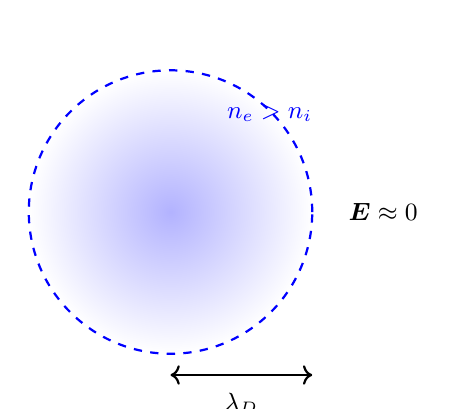
\begin{tikzpicture}[scale=0.9]
\fill[red] (0,0) circle (4pt);
\node[red, font=\small] at (0,0.5) {$+Q$};
\shade[inner color=blue!30, outer color=white] (0,0) circle (2);
\draw[dashed, blue, thick] (0,0) circle (2);
\node[blue, font=\small] at (1.4,1.4) {$n_e > n_i$};
\node[font=\small] at (3,0) {$\vect{E}\approx 0$};
\draw[<->, thick] (0,-2.3) -- (2,-2.3);
\node[font=\small] at (1,-2.7) {$\lambda_D$};
\end{tikzpicture}
\end{center}

\subsection{定量推导}

\begin{theorem}{德拜长度}{debye-length}
在温度为 $T$、数密度为 $n$ 的热平衡等离子体中，德拜长度为：
\[
\lambda_D = \sqrt{\frac{\eps_0 k_B T}{n e^2}}
\]
对电子和离子分别定义：
\[
\lambda_{De} = \sqrt{\frac{\eps_0 k_B T_e}{n_e e^2}}, \qquad \lambda_{Di} = \sqrt{\frac{\eps_0 k_B T_i}{n_i e^2}}
\]
总德拜长度满足：
\[
\frac{1}{\lambda_D^2} = \frac{1}{\lambda_{De}^2} + \frac{1}{\lambda_{Di}^2}
\]
\end{theorem}

\begin{proof}[推导思路]
考虑等离子体中插入一个试探正电荷，设产生的电势为 $\phi(r)$。电子和离子在该电势中的密度服从玻尔兹曼分布：
\[
n_e = n_0 \exp\left(\frac{e\phi}{k_B T_e}\right), \qquad n_i = n_0 \exp\left(-\frac{e\phi}{k_B T_i}\right)
\]
在小电势近似 $e\phi \ll k_B T$ 下展开：
\[
n_e \approx n_0\left(1 + \frac{e\phi}{k_B T_e}\right), \qquad n_i \approx n_0\left(1 - \frac{e\phi}{k_B T_i}\right)
\]
空间电荷密度：
\[
\rho = e(n_i - n_e) \approx -en_0\left(\frac{e\phi}{k_B T_e} + \frac{e\phi}{k_B T_i}\right) = -\frac{\eps_0}{\lambda_D^2}\phi
\]
代入泊松方程 $\lap\phi = -\rho/\eps_0$：
\[
\lap\phi = \frac{\phi}{\lambda_D^2}
\]
在球坐标下，考虑球对称解，令 $u=r\phi$，则方程变为：
\[
\frac{\diff^2 u}{\diff r^2} = \frac{u}{\lambda_D^2}
\]
满足边界条件 $\phi(\infty)=0$ 和 $r\to 0$ 时趋于点电荷电势的解为：
\[
\phi(r) = \frac{Q}{4\pi\eps_0 r} \exp\left(-\frac{r}{\lambda_D}\right)
\]
这就是德拜屏蔽势——在 $r \gg \lambda_D$ 时指数衰减。
\end{proof}

\begin{insight}{德拜屏蔽的物理意义}{debye-insight}
德拜屏蔽揭示了等离子体的三个核心属性：
\begin{enumerate}
\item \textbf{准中性}：在远大于 $\lambda_D$ 的尺度上，等离子体是电中性的。任何电荷不平衡只能局域在德拜球以内。
\item \textbf{集体行为}：屏蔽不是单个电子完成的，而是大量电子在热运动背景下通过长程库仑相互作用协同完成的。
\item \textbf{对试探电荷的响应}：德拜长度决定了等离子体对外部扰动的"感知范围"。
\end{enumerate}
\end{insight}

\begin{example}{计算德拜长度}{debye-calc}
\difficulty{基础}
一实验室等离子体参数为 $n_e = 10^{18}\,\mathrm{m}^{-3}$，$T_e = 2\,\mathrm{eV}$（约 $2.3\times 10^4\,\mathrm{K}$）。求电子德拜长度和德拜球内的粒子数。
\tcblower
\textbf{解答：}

首先将温度转换为焦耳：$k_B T_e = 2\,\mathrm{eV} = 2 \times 1.602\times 10^{-19}\,\mathrm{J} = 3.204\times 10^{-19}\,\mathrm{J}$。

\[
\lambda_{De} = \sqrt{\frac{\eps_0 k_B T_e}{n_e e^2}} = \sqrt{\frac{(8.854\times 10^{-12})(3.204\times 10^{-19})}{(10^{18})(1.602\times 10^{-19})^2}}
\]
计算分子：$8.854\times 10^{-12} \times 3.204\times 10^{-19} \approx 2.836\times 10^{-30}$

计算分母：$10^{18} \times 2.566\times 10^{-38} = 2.566\times 10^{-20}$

\[
\lambda_{De} = \sqrt{\frac{2.836\times 10^{-30}}{2.566\times 10^{-20}}} \approx \sqrt{1.105\times 10^{-10}} \approx 1.05\times 10^{-5}\,\mathrm{m} \approx 10.5\,\mu\mathrm{m}
\]

德拜球体积：
\[
V_D = \frac{4}{3}\pi \lambda_{De}^3 \approx \frac{4}{3}\pi (10.5\times 10^{-6})^3 \approx 4.85\times 10^{-15}\,\mathrm{m}^3
\]

德拜球内粒子数：
\[
N_D = n_e V_D \approx 10^{18} \times 4.85\times 10^{-15} \approx 4.85\times 10^{3}
\]
约5000个粒子——远大于1，说明集体屏蔽确实成立。
\end{example}

\section{等离子体频率}\difficulty{基础}

\begin{definition}{电子等离子体频率}{plasma-freq-def}
电子等离子体频率定义为：
\[
\omega_{pe} = \sqrt{\frac{n_e e^2}{\eps_0 m_e}}
\]
对应的离子等离子体频率为：
\[
\omega_{pi} = \sqrt{\frac{n_i Z^2 e^2}{\eps_0 m_i}}
\]
其中 $Z$ 是离子电荷数。由于 $m_i \gg m_e$，通常 $\omega_{pi} \ll \omega_{pe}$。
\end{definition}

\begin{insight}{等离子体频率的物理图像}{wp-insight}
等离子体频率有一个简洁的物理推导：假设等离子体中电子整体相对于固定离子背景发生了微小位移 $\Delta x$。这产生一个面电荷密度 $\sigma = n_e e \Delta x$，对应的电场 $E = \sigma/\eps_0 = n_e e \Delta x/\eps_0$。电子受到的恢复力为 $-eE$，运动方程为：
\[
m_e \ddot{\Delta x} = -\frac{n_e e^2}{\eps_0}\Delta x
\]
这是简谐振动方程，频率正是 $\omega_{pe}$。

这说明：等离子体会以特征频率 $\omega_{pe}$ 对外部扰动作"弹性"响应。任何频率低于 $\omega_{pe}$ 的电磁信号都无法穿透等离子体——这就是金属对低频电磁波的反射机制，也是电离层反射无线电波的原理。
\end{insight}

\begin{example}{典型等离子体的频率与德拜长度}{typical-params}
\difficulty{基础}
填写下表中典型等离子体环境的参数估算（数量级即可）。
\begin{center}
\begin{tabular}{lcccc}
\toprule
\textbf{环境} & $n_e\,(\mathrm{m}^{-3})$ & $T_e\,(\mathrm{eV})$ & $\lambda_D\,(\mathrm{m})$ & $\omega_{pe}\,(\mathrm{rad/s})$ \\
\midrule
星际介质 & $10^6$ & $10^{-2}$ & $10$ & $10^4$ \\
电离层 & $10^{12}$ & $10^{-1}$ & $10^{-3}$ & $10^7$ \\
实验室等离子体 & $10^{18}$ & $10$ & $10^{-5}$ & $10^{11}$ \\
惯性约束聚变 & $10^{32}$ & $10^4$ & $10^{-10}$ & $10^{18}$ \\
\bottomrule
\end{tabular}
\end{center}
\tcblower
\textbf{分析}：

从表中可见，等离子体参数跨越了\textbf{超过20个数量级}！但无论密度和温度如何变化，等离子体的两个关键无量纲参数——德拜球内粒子数 $N_D$ 和耦合参数 $\Gamma$——才是判断系统是否为"真等离子体"的核心。
\end{example}

\section{等离子体判据}\difficulty{基础}

一种电离气体要被称为等离子体，必须满足三个基本条件。

\begin{theorem}{等离子体的三个判据}{plasma-criteria}
设系统尺度为 $L$，粒子数为 $N$，德拜球内粒子数为 $N_D$，耦合参数为 $\Gamma$。

\textbf{判据一}（准中性尺度）：
\[
L \gg \lambda_D
\]
系统尺度远大于德拜长度，才能保证大尺度准中性。

\textbf{判据二}（集体行为）：
\[
N_D = n\lambda_D^3 \gg 1
\]
德拜球内包含大量粒子，屏蔽是集体效应而非少数粒子的行为。

\textbf{判据三}（弱耦合）：
\[
\Gamma = \frac{e^2}{4\pi\eps_0 a k_B T} \ll 1
\]
其中 $a \sim n^{-1/3}$ 是粒子平均间距。粒子热动能远大于库仑相互作用能，系统处于弱耦合状态。
\end{theorem}

\begin{insight}{耦合参数的直观含义}{gamma-insight}
耦合参数 $\Gamma$ 是粒子间的典型库仑势能 $e^2/4\pi\eps_0 a$ 与典型热动能 $k_BT$ 之比：
\begin{itemize}
\item $\Gamma \ll 1$（\textbf{弱耦合}）：粒子热运动剧烈，库仑相互作用只是微扰。大多数实验室等离子体、空间等离子体属于此类。
\item $\Gamma \sim 1$（\textbf{强耦合边界}）：粒子开始"感受"到彼此的存在，关联效应变得重要。
\item $\Gamma \gg 1$（\textbf{强耦合}）：库仑势能占主导，粒子形成有序结构（如库仑晶体）。白矮星内部、极稠密激光等离子体、尘埃等离子体中可能出现。
\end{itemize}
\end{insight}

\begin{history}{朗缪尔探针与等离子体诊断的诞生}{langmuir-history}
1924年，朗缪尔在研究汞蒸气放电时发明了以他名字命名的\textbf{朗缪尔探针}（Langmuir Probe）——一根插入等离子体的小金属丝，通过改变其偏压测量电流--电压特性曲线。这是人类历史上第一种等离子体诊断工具，至今仍在广泛使用。朗缪尔探针可以测量电子温度、电子密度和等离子体电势，原理正是基于德拜屏蔽和玻尔兹曼关系。有趣的是，朗缪尔还发现了"等离子体鞘层"（Sheath）现象：探针表面附近会形成一个薄的非中性区域，其厚度约为几个德拜长度——这正是判据一 $L \gg \lambda_D$ 的直接体现。
\end{history}

\begin{warning}{"电离气体"不等于"等离子体"}{ionized-not-plasma}
以下情况虽然包含带电粒子，但\textbf{不是}等离子体：
\begin{enumerate}
\item \textbf{极稀薄电离气体}：如 $n=10^3\,\mathrm{m}^{-3}$、$T=10^6\,\mathrm{K}$ 的某些星际区域。虽然 $T$ 很高，但 $N_D \ll 1$，德拜屏蔽不成立。
\item \textbf{极稠密强耦合系统}：如固体中的传导电子（金属），$\Gamma \gg 1$，需要用能带理论而非等离子体物理描述。
\item \textbf{中性气体中的少量离子}：如刚点火的荧光灯管，电离度极低，带电粒子主要与中性原子碰撞，不表现集体行为。
\end{enumerate}
\end{warning}

\begin{chapterreview}
\begin{itemize}
\item \textbf{德拜长度} $\lambda_D = \sqrt{\eps_0 k_BT/ne^2}$ 是等离子体的特征屏蔽尺度，也是准中性的最小尺度。
\item \textbf{等离子体频率} $\omega_{pe} = \sqrt{n_e e^2/\eps_0 m_e}$ 是电子对电荷不平衡的集体响应频率。
\item 等离子体的\textbf{三个判据}：$L \gg \lambda_D$、$N_D \gg 1$、$\Gamma \ll 1$（弱耦合）。
\item 德拜屏蔽势：$\phi(r) = (Q/4\pi\eps_0 r)\ee^{-r/\lambda_D}$，在 $r>\lambda_D$ 时指数衰减。
\item 等离子体参数空间跨越20多个数量级，但核心物理（集体行为、准中性）不变。
\end{itemize}
\end{chapterreview}

\begin{miniquiz}
\begin{enumerate}
\item 某等离子体 $n_e = 10^{16}\,\mathrm{m}^{-3}$，$T_e = 1\,\mathrm{eV}$，求 $\lambda_{De}$ 和 $\omega_{pe}$。
\item 为什么 $\omega_{pi} \ll \omega_{pe}$？从物理上解释。
\item 如果一种电离气体的 $N_D \approx 0.5$，它是否能被称为等离子体？为什么？
\item 德拜屏蔽是否意味着等离子体内部完全没有电场？如果不是，在什么尺度上电场可以被忽略？
\end{enumerate}
\end{miniquiz}


% ============================================================
% 第3章：单粒子运动
% ============================================================
\chapter{单粒子运动}
\epigraph{在理解集体行为之前，先理解单个粒子的舞蹈。}{--- 弗兰西斯·切恩（Francis F. Chen）}

\begin{insight}{本章核心目标}{ch3-goal}
掌握带电粒子在均匀及非均匀电磁场中的运动规律——回旋运动、$\vect{E}\times\vect{B}$ 漂移、梯度漂移、曲率漂移、磁镜效应。理解"导向中心近似"的思想，这是连接单粒子图像与流体图像的桥梁。
\tcblower
\textbf{学习路径建议：}

\begin{itemize}[leftmargin=*]
\item[\textcolor{red}{$\blacksquare$}] \textbf{必学}：\S3.1 均匀磁场中的回旋运动；\S3.2 $\vect{E}\times\vect{B}$ 漂移；\S3.3 非均匀磁场中的梯度漂移与曲率漂移
\item[\textcolor{orange}{$\blacksquare$}] \textbf{重要}：\S3.4 磁镜效应与磁瓶约束；\S3.5 绝热不变量
\item[\textcolor{green}{$\blacksquare$}] \textbf{可延后}：\S3.6 导向中心运动的系统推导（高阶漂移）
\end{itemize}
\end{insight}

等离子体是大量带电粒子的集合。最朴素的出发点是：先忽略粒子之间的相互作用，只研究\textbf{单个粒子在外加电磁场中的运动}。这看似过于简化，但实际上：
\begin{itemize}
\item 高频行为（$\omega \gg \omega_{pi}$）中离子来不及响应，电子的运动近似于单粒子行为；
\item 在强磁场、低密度条件下，粒子间的库仑碰撞稀少，单粒子图像十分准确；
\item 单粒子运动的漂移速度直接进入了MHD方程（第5章），是理解宏观约束的关键。
\end{itemize}

\section{均匀磁场中的回旋运动}\difficulty{基础}

\begin{theorem}{带电粒子在均匀磁场中的运动}{gyromotion}
设磁场 $\vect{B} = B_0\unitvec{z}$ 均匀且恒定，无电场。电荷为 $q$、质量为 $m$ 的粒子运动方程为：
\[
m\frac{\diff\vect{v}}{\diff t} = q\vect{v}\times\vect{B}
\]
解由两部分组成：

\textbf{平行于磁场的运动}（$z$方向）：
\[
v_z = v_{\parallel} = \text{常数}
\]
粒子以恒定速度沿磁力线自由运动。

\textbf{垂直于磁场的运动}（$xy$平面）：
粒子做匀速圆周运动——\textbf{回旋运动（Gyration）}：
\begin{align*}
v_x &= v_\perp \cos(\omega_c t + \phi_0) \\
v_y &= -\frac{q}{|q|} v_\perp \sin(\omega_c t + \phi_0)
\end{align*}
其中回旋频率（Cyclotron Frequency）为：
\[
\omega_c = \frac{|q|B_0}{m}
\]
回旋半径（Larmor Radius）为：
\[
\rho_L = \frac{v_\perp}{\omega_c} = \frac{m v_\perp}{|q|B_0}
\]
\end{theorem}

\begin{insight}{回旋运动的物理图像}{gyro-insight}
洛伦兹力 $q\vect{v}\times\vect{B}$ 始终垂直于速度方向，因此不做功，只改变速度方向。粒子在垂直于磁场的平面内划出完美的圆，同时以恒定速度沿磁场方向"滑行"。整体轨迹是一条\textbf{螺旋线}。

旋转方向由电荷符号决定：正电荷逆时针旋转（从磁场方向看），负电荷顺时针。在等离子体中，电子的回旋频率远高于离子（$\omega_{ce}/\omega_{ci} = m_i/m_e \sim 10^3$--$10^5$），而回旋半径则远小于离子（$\rho_{Le}/\rho_{Li} = \sqrt{m_e T_e/m_i T_i} \ll 1$）。
\end{insight}

\begin{center}
\begin{tikzpicture}[scale=0.85]
\foreach \x in {-2,-1,0,1,2} {
  \foreach \y in {-2,-1,0,1,2} {
    \draw[->, green!50!black, line width=0.6pt] (\x,\y,-2) -- (\x,\y,2);
  }
}
\node[green!50!black, font=\small] at (3,0,0) {$\vect{B}$};
\draw[red, thick, domain=0:720, samples=100, variable=\t]
  plot({1.2*cos(-\t+90)}, {1.2*sin(-\t+90)}, {\t/180});
\node[red, font=\small] at (1.5,1.5,2) {电子};
\draw[blue, thick, domain=0:720, samples=100, variable=\t]
  plot({1.5*cos(\t)}, {1.5*sin(\t)}, {\t/180});
\node[blue, font=\small] at (-1.5,-1.5,2) {离子};
\end{tikzpicture}
\end{center}

\begin{example}{计算典型回旋参数}{gyro-calc}
\difficulty{基础}
托卡马克中典型参数：$B = 5\,\mathrm{T}$，$T_e = 10\,\mathrm{keV}$，$T_i = 10\,\mathrm{keV}$（氘离子）。求电子和离子的回旋频率与回旋半径。
\tcblower
\textbf{解答：}

电子回旋频率：
\[
\omega_{ce} = \frac{eB}{m_e} = \frac{(1.602\times 10^{-19})(5)}{9.109\times 10^{-31}} \approx 8.8\times 10^{11}\,\mathrm{rad/s}
\]
对应频率 $f_{ce} = \omega_{ce}/2\pi \approx 1.4\times 10^{11}\,\mathrm{Hz}$（140 GHz，毫米波段）。

电子热速度：
\[
v_{te} = \sqrt{\frac{k_B T_e}{m_e}} = \sqrt{\frac{(10^4)(1.602\times 10^{-19})}{9.109\times 10^{-31}}} \approx 1.33\times 10^{8}\,\mathrm{m/s}
\]
电子回旋半径：
\[
\rho_{Le} = \frac{v_{te}}{\omega_{ce}} \approx \frac{1.33\times 10^8}{8.8\times 10^{11}} \approx 1.5\times 10^{-4}\,\mathrm{m} = 0.15\,\mathrm{mm}
\]

对于氘离子（$m_i \approx 2\times 1.673\times 10^{-27}\,\mathrm{kg} = 3.346\times 10^{-27}\,\mathrm{kg}$）：
\[
\omega_{ci} = \frac{eB}{m_i} \approx 2.4\times 10^{8}\,\mathrm{rad/s}, \qquad f_{ci} \approx 38\,\mathrm{MHz}
\]
\[
v_{ti} = \sqrt{\frac{k_B T_i}{m_i}} \approx 2.2\times 10^{6}\,\mathrm{m/s}, \qquad \rho_{Li} = \frac{v_{ti}}{\omega_{ci}} \approx 9\,\mathrm{mm}
\]
可见离子回旋半径约为电子的60倍，但仍远小于装置尺度（托卡马克大半径约 $1$--$2\,\mathrm{m}$）。
\end{example}

\section{电场与磁场交叉：漂移运动}\difficulty{基础}

当同时存在电场和磁场时，粒子的运动不再是简单的螺旋线，其导向中心（回旋圆的中心）会发生\textbf{漂移}。

\subsection{E×B 漂移}

\begin{theorem}{$\vect{E}\times\vect{B}$ 漂移}{exb-drift}
在均匀电磁场 $\vect{E}$ 和 $\vect{B}$ 中（设 $\vect{E}\perp\vect{B}$），粒子的导向中心以恒定速度漂移：
\[
\vect{v}_E = \frac{\vect{E}\times\vect{B}}{B^2}
\]
关键性质：
\begin{itemize}
\item 漂移速度与电荷 $q$ 和质量 $m$ 均无关
\item 电子和离子以相同速度和方向漂移，因此不会引起净电流
\item 漂移方向垂直于 $\vect{E}$ 和 $\vect{B}$，遵循右手定则
\end{itemize}
\end{theorem}

\begin{proof}[推导]
运动方程为 $m\dot{\vect{v}} = q(\vect{E} + \vect{v}\times\vect{B})$。将速度分解为回旋运动和漂移：$\vect{v} = \vect{v}' + \vect{v}_E$，其中 $\vect{v}_E$ 是待求的常数漂移速度。代入方程：
\[
m\dot{\vect{v}'} = q(\vect{E} + (\vect{v}' + \vect{v}_E)\times\vect{B}) = q\vect{E} + q\vect{v}'\times\vect{B} + q\vect{v}_E\times\vect{B}
\]
若选择 $\vect{v}_E$ 使得常数项为零：
\[
\vect{E} + \vect{v}_E\times\vect{B} = 0
\]
两边叉乘 $\vect{B}$：
\[
\vect{E}\times\vect{B} + (\vect{v}_E\times\vect{B})\times\vect{B} = 0
\]
利用矢量恒等式 $(\vect{A}\times\vect{B})\times\vect{B} = -B^2\vect{A}_\perp$（这里 $\vect{E}\perp\vect{B}$，所以 $\vect{E}$ 已经是垂直分量）：
\[
\vect{E}\times\vect{B} - B^2\vect{v}_E = 0 \quad\Rightarrow\quad \vect{v}_E = \frac{\vect{E}\times\vect{B}}{B^2}
\]
此时方程退化为 $m\dot{\vect{v}'} = q\vect{v}'\times\vect{B}$，即纯粹的回旋运动。证毕。
\end{proof}

\begin{insight}{$\vect{E}\times\vect{B}$ 漂移的物理图像}{exb-insight}
想象一个正离子在磁场中做回旋运动。当它逆着电场方向运动时，电场对其做负功，速度减小，回旋半径变小；当它顺着电场方向运动时，电场做正功，速度增大，回旋半径变大。结果：轨迹不再是闭合圆，而是形成一个"摆线"——整体向 $\vect{E}\times\vect{B}$ 方向漂移。

由于漂移速度与 $q$ 无关，电子和离子的漂移方向相同。这一点极其重要：$\vect{E}\times\vect{B}$ 漂移不会导致电荷分离！
\end{insight}

\begin{warning}{$\vect{E}\times\vect{B}$ 漂移的常见误区}{exb-mistake}
\begin{enumerate}
\item 误以为 $\vect{v}_E$ 与 $q$ 有关。实际上它是\textbf{电磁场的几何属性}，任何粒子都以相同速度漂移。
\item 当 $\vect{E}$ 有平行于 $\vect{B}$ 的分量时，粒子会沿磁场加速（$F_\parallel = qE_\parallel$），同时垂直方向仍有 $\vect{E}\times\vect{B}$ 漂移。两部分运动独立叠加。
\item 漂移速度的大小 $v_E = E/B$。若 $E > cB$（在自然单位制下），则 $v_E > c$，这看似超光速悖论，实则因为此时参考系变换下的电磁场描述需要相对论处理，$\vect{E}\times\vect{B}$ 漂移公式本身仅在非相对论条件下成立。
\end{enumerate}
\end{warning}

\subsection{梯度漂移与曲率漂移}

当磁场非均匀时，会出现两种新的漂移。

\begin{theorem}{梯度漂移与曲率漂移}{grad-curv-drift}
设磁场方向基本沿 $z$，但存在弱的横向梯度和曲率。

\textbf{梯度漂移}（由磁场强度梯度 $\grad B$ 引起）：
\[
\vect{v}_{\nabla B} = \frac{\mu}{qB^2}(\vect{B}\times\grad B) = \frac{m v_\perp^2}{2qB^3}(\vect{B}\times\grad B)
\]
其中 $\mu = mv_\perp^2/2B$ 是磁矩（见\S3.5）。

\textbf{曲率漂移}（由磁力线弯曲引起）：
\[
\vect{v}_R = \frac{m v_\parallel^2}{qB^2 R_c^2}(\vect{R}_c\times\vect{B})
\]
其中 $\vect{R}_c$ 是曲率半径矢量，指向曲率中心。

两种漂移的方向均依赖于电荷符号 $q$，因此电子和离子反向漂移，会产生净电流！
\end{theorem}

\begin{insight}{梯度漂移与曲率漂移的物理根源}{grad-curv-insight}
梯度漂移的物理图像与 $\vect{E}\times\vect{B}$ 漂移类似：在磁场较强的区域，回旋半径较小；在磁场较弱的区域，回旋半径较大。粒子轨迹因此产生整体漂移。

曲率漂移则源于离心力。当粒子沿弯曲的磁力线运动时，会受到离心力 $m v_\parallel^2/R_c$ 的作用，这个等效"力"导致了与 $\vect{F}\times\vect{B}/qB^2$ 形式相同的漂移。
\end{insight}

\section{磁镜与磁瓶约束}\difficulty{提高}

\begin{theorem}{磁矩守恒与磁镜效应}{magnetic-mirror}
在缓慢变化的磁场中（变化尺度远大于回旋半径），粒子的\textbf{磁矩}：
\[
\mu = \frac{m v_\perp^2}{2B}
\]
是一个\textbf{绝热不变量}（近似守恒量）。

若粒子从弱磁场区 $B_{\min}$ 向强磁场区 $B_{\max}$ 运动，由于 $\mu$ 守恒，$v_\perp$ 随 $B$ 增大而增大。因总动能守恒，$v_\parallel$ 必须减小。若 $B_{\max}$ 足够大，使得 $v_\parallel \to 0$ 时粒子尚未到达 $B_{\max}$，则粒子会被"反射"回去——这就是\textbf{磁镜效应}。

反射条件（损失锥）：
\[
\sin^2\theta > \frac{B_{\min}}{B_{\max}} \equiv \frac{1}{R_m}
\]
其中 $\theta$ 是粒子在 $B_{\min}$ 处的俯仰角，$R_m$ 是磁镜比。不满足此条件的粒子将穿过磁镜而损失。
\end{theorem}

\begin{insight}{磁镜在自然界与实验室中的应用}{mirror-insight}
\textbf{地球磁层}就是天然的磁瓶：带电粒子被地磁场捕获，在南北磁极之间来回反射，形成范艾伦辐射带。太阳风中的粒子进入磁层后，也会沿着磁力线沉降到极区大气，与氧原子碰撞产生绚丽的\textbf{极光}。

\textbf{实验室磁镜装置}曾是最早的磁约束聚变方案之一。但由于损失锥中的粒子始终会逃逸，简单的磁镜存在\textbf{终端损失}问题。后来发展出的\textbf{串列磁镜}（Tandem Mirror）和\textbf{仿星器}（Stellarator）通过更复杂的磁场位形来缓解这一问题。
\end{insight}

\begin{chapterreview}
\begin{itemize}
\item 均匀磁场中粒子做\textbf{回旋运动}：$\omega_c = |q|B/m$，$\rho_L = mv_\perp/|q|B$。
\item $\vect{E}\times\vect{B}$ 漂移：$\vect{v}_E = \vect{E}\times\vect{B}/B^2$，与 $q$ 无关。
\item 梯度漂移和曲率漂移与 $q$ 有关，电子离子反向，产生净电流。
\item \textbf{磁矩} $\mu = mv_\perp^2/2B$ 是绝热不变量，导致磁镜反射。
\item 磁镜比 $R_m = B_{\max}/B_{\min}$ 决定损失锥角度。
\end{itemize}
\end{chapterreview}

\begin{miniquiz}
\begin{enumerate}
\item 证明：若 $\vect{E}$ 有平行于 $\vect{B}$ 的分量，则 $\vect{E}\times\vect{B}$ 漂移公式仍然成立，只是粒子 additionally 沿磁场加速。
\item 为什么梯度漂移会产生净电流，而 $\vect{E}\times\vect{B}$ 漂移不会？
\item 一电子在 $B=1\,\mathrm{T}$ 磁场中，$T_e=100\,\mathrm{eV}$。求其回旋半径和回旋频率。
\item 解释为什么磁镜可以约束粒子，但无法约束一个零温度的冷等离子体（所有粒子 $v_\perp=0$）。
\end{enumerate}
\end{miniquiz}



% ============================================================
% 第4章：流体描述基础
% ============================================================
\chapter{流体描述基础}
\epigraph{当粒子数足够多时，统计规律就会战胜个体的任性。}{--- 路德维希·玻尔兹曼}

\begin{insight}{本章核心目标}{ch4-goal}
从玻尔兹曼方程出发，通过取矩得到等离子体的流体方程组——连续性方程、运动方程和能量方程。建立双流体模型，理解电子和离子可以具有不同的温度和流速。
\tcblower
\textbf{学习路径建议：}

\begin{itemize}[leftmargin=*]
\item[\textcolor{red}{$\blacksquare$}] \textbf{必学}：\S4.1 玻尔兹曼方程与矩方程；\S4.2 双流体方程组；\S4.3 广义欧姆定律
\item[\textcolor{orange}{$\blacksquare$}] \textbf{重要}：\S4.4 状态方程与闭合问题
\item[\textcolor{green}{$\blacksquare$}] \textbf{可延后}：\S4.5 碰撞项的简化模型（用到时回看）
\end{itemize}
\end{insight}

单粒子图像虽然优美，但当我们要处理 $10^{18}$ 个粒子时，逐一枚举它们的轨道是不现实的。流体描述的本质是：在比德拜长度大、比等离子体频率周期长的时空尺度上，粒子系统的宏观平均行为可以用类似普通流体的方程来描述。

\section{玻尔兹曼方程}\difficulty{基础}

\begin{definition}{玻尔兹曼方程}{boltzmann-def}
分布函数 $f(\vect{r},\vect{v},t)$ 的演化满足玻尔兹曼方程：
\[
\frac{\partial f}{\partial t} + \vect{v}\cdot\grad f + \frac{\vect{F}}{m}\cdot\grad_v f = \left(\frac{\partial f}{\partial t}\right)_c
\]
其中 $\vect{F} = q(\vect{E} + \vect{v}\times\vect{B})$ 是洛伦兹力，$\grad_v = \partial/\partial\vect{v}$ 是速度空间的梯度算子，右端 $(\partial f/\partial t)_c$ 是碰撞项。
\end{definition}

\begin{insight}{玻尔兹曼方程各项的物理意义}{boltzmann-insight}
\begin{itemize}
\item $\partial f/\partial t$：分布函数随时间的局域变化
\item $\vect{v}\cdot\grad f$：粒子以速度 $\vect{v}$ 运动带来的空间输运（对流项）
\item $(\vect{F}/m)\cdot\grad_v f$：外力（电磁力）引起粒子在速度空间中的"流动"
\item 碰撞项：短程碰撞导致粒子在速度空间中重新分布
\end{itemize}
左端三项合起来可以写成全导数形式：
\[
\frac{\diff f}{\diff t} = \frac{\partial f}{\partial t} + \vect{v}\cdot\grad f + \frac{\vect{F}}{m}\cdot\grad_v f
\]
这是相空间中随粒子一起运动的观察者看到的分布函数变化率。
\end{insight}

\section{矩方程的推导}\difficulty{提高}

通过对玻尔兹曼方程乘以 $\vect{v}$ 的不同幂次并积分，可以得到宏观量的演化方程。

\subsection{零阶矩：连续性方程}

将玻尔兹曼方程对速度空间积分（即取零阶矩）：
\[
\int \frac{\partial f}{\partial t}\,\diff^3v + \int \vect{v}\cdot\grad f\,\diff^3v + \int \frac{\vect{F}}{m}\cdot\grad_v f\,\diff^3v = \int \left(\frac{\partial f}{\partial t}\right)_c \diff^3v
\]

利用分布函数在速度无穷远处为零的边界条件，可以证明第三项（力项）积分为零（因为力只改变速度方向，不改变粒子总数），碰撞项也保持粒子总数不变（质量守恒）。最终得到：

\begin{theorem}{连续性方程}{continuity}
\[
\frac{\partial n}{\partial t} + \divg(n\vect{u}) = 0
\]
或等价地：
\[
\frac{\partial n}{\partial t} + \vect{u}\cdot\grad n + n\divg\vect{u} = 0
\]
物理意义：某点粒子数密度的变化 = 流入的粒子 $-$ 流出的粒子。这是质量守恒的局域表达。
\end{theorem}

\subsection{一阶矩：运动方程}

将玻尔兹曼方程乘以 $m\vect{v}$ 再积分，经过一系列运算（需要引入压强张量的定义），得到：

\begin{theorem}{运动方程（动量方程）}{momentum-eq}
\[
nm\left(\frac{\partial\vect{u}}{\partial t} + \vect{u}\cdot\grad\vect{u}\right) = qn(\vect{E} + \vect{u}\times\vect{B}) - \grad\cdot\bm{P} + \vect{R}
\]
其中：
\begin{itemize}
\item 左端是流体元的惯性力（质量乘以加速度）
\item 右端第一项是电磁体积力
\item $\bm{P}$ 是压强张量，$\grad\cdot\bm{P}$ 是其散度（力的密度）
\item $\vect{R}$ 是碰撞导致的动量交换（与其他种类的粒子碰撞时）
\end{itemize}
\end{theorem}

\begin{insight}{压强张量的物理意义}{pressure-tensor}
压强张量 $P_{ij}$ 描述的是动量流：$P_{ij}$ 表示单位时间内通过垂直于 $j$ 方向的单位面积，沿 $i$ 方向输运的动量。对于各向同性的热分布，$P_{ij} = p\delta_{ij}$，此时 $-\grad\cdot\bm{P} = -\grad p$，即普通流体中的压强梯度力。

在磁化等离子体中，由于磁场使粒子运动各向异性（平行和垂直磁场方向的行为不同），压强张量通常具有双绝热形式：
\[
\bm{P} = p_\perp\bm{I} + (p_\parallel - p_\perp)\frac{\vect{B}\vect{B}}{B^2}
\]
其中 $\vect{B}\vect{B}$ 是并矢。$p_\parallel$ 和 $p_\perp$ 分别对应平行和垂直于磁场的压强分量。
\end{insight}

\section{双流体方程组}\difficulty{提高}

等离子体至少包含两种带电粒子：电子和离子。由于 $m_e \ll m_i$，在很多现象中电子和离子的响应完全不同，必须分别描述。

\begin{theorem}{双流体方程组}{two-fluid}
对每种粒子种类 $\alpha$（$\alpha = e$ 电子，$\alpha = i$ 离子），有：

\textbf{连续性方程}：
\[
\frac{\partial n_\alpha}{\partial t} + \divg(n_\alpha\vect{u}_\alpha) = 0
\]

\textbf{运动方程}：
\[
n_\alpha m_\alpha\left(\frac{\partial\vect{u}_\alpha}{\partial t} + \vect{u}_\alpha\cdot\grad\vect{u}_\alpha\right) = n_\alpha q_\alpha(\vect{E} + \vect{u}_\alpha\times\vect{B}) - \grad p_\alpha + \vect{R}_\alpha
\]

\textbf{状态方程（理想气体）}：
\[
p_\alpha = n_\alpha k_B T_\alpha
\]

\textbf{麦克斯韦方程组}（自洽场）：
\begin{align*}
\divg\vect{E} &= \frac{\rho}{\eps_0} = \frac{e(n_i - n_e)}{\eps_0} \\
\divg\vect{B} &= 0 \\
\curl\vect{E} &= -\frac{\partial\vect{B}}{\partial t} \\
\curl\vect{B} &= \mu_0\vect{j} + \mu_0\eps_0\frac{\partial\vect{E}}{\partial t}, \quad \vect{j} = e(n_i\vect{u}_i - n_e\vect{u}_e)
\end{align*}
\end{theorem}

\begin{insight}{双流体模型的物理内涵}{two-fluid-insight}
双流体模型捕捉了等离子体的一个核心特征：\textbf{电子和离子可以脱耦}。由于电子质量小，它们能迅速响应电场变化；而离子惯性大，响应慢得多。这种质量差异导致了丰富的物理现象：
\begin{itemize}
\item 高频波（$\omega \sim \omega_{pe}$）中离子基本不动，只有电子振荡（Langmuir波）
\item 低频波（$\omega \ll \omega_{ci}$）中电子和离子一起运动，表现为单流体（MHD，第5章）
\item 中间频率范围出现离子声波、低混杂波等双流体特有的模式
\end{itemize}
\end{insight}

\section{广义欧姆定律}\difficulty{提高}

从双流体方程可以导出一个极为重要的关系——将电流密度 $\vect{j}$ 与电场 $\vect{E}$ 联系起来的方程。

\begin{theorem}{广义欧姆定律}{ohms-law}
在准中性 ($n_e = n_i = n$)、非相对论条件下，电流密度的演化满足：
\[
\vect{E} + \vect{u}\times\vect{B} = \eta\vect{j} + \frac{1}{en}\vect{j}\times\vect{B} - \frac{1}{en}\grad p_e + \frac{m_e}{n e^2}\frac{\partial\vect{j}}{\partial t}
\]
其中 $\vect{u}$ 是质心速度，$\eta$ 是电阻率。

各项的物理意义：
\begin{itemize}
\item $\vect{E} + \vect{u}\times\vect{B}$：在随流体运动的参考系中的有效电场
\item $\eta\vect{j}$：电阻（欧姆）项
\item $\dfrac{1}{en}\vect{j}\times\vect{B}$：\textbf{霍尔项}，反映电子和离子在磁场中的不同偏转
\item $-\dfrac{1}{en}\grad p_e$：\textbf{电子压强梯度项}（双极扩散的来源）
\item $\dfrac{m_e}{ne^2}\dfrac{\partial\vect{j}}{\partial t}$：\textbf{电子惯性项}（高频时重要）
\end{itemize}
\end{theorem}

\begin{history}{欧姆定律的等离子体推广}{ohms-history}
乔治·欧姆在1827年提出著名的 $V=IR$ 时，研究的是固态导体中的电流。在等离子体中，由于存在自由电子、磁场和压强梯度，简单的欧姆定律远远不够。等离子体版本的广义欧姆定律最早由斯必泽（Lyman Spitzer）等人在20世纪50年代系统导出，是磁流体力学和等离子体输运理论的基石。其中霍尔项的存在意味着：即使在理想导体（$\eta=0$）中，电流也可以由磁场和压强梯度"驱动"——这与普通电路中的欧姆定律截然不同。
\end{history}

\begin{chapterreview}
\begin{itemize}
\item 玻尔兹曼方程描述分布函数的演化，碰撞项体现粒子间短程相互作用。
\item 取矩得到\textbf{连续性方程}（质量守恒）和\textbf{运动方程}（动量守恒）。
\item \textbf{双流体模型}分别描述电子和离子，捕捉质量差异导致的脱耦行为。
\item \textbf{广义欧姆定律}联系 $\vect{j}$ 与 $\vect{E}$，包含电阻、霍尔、压强梯度和惯性四项。
\item 等离子体方程组需要\textbf{闭合条件}（状态方程）才能求解。
\end{itemize}
\end{chapterreview}

\begin{miniquiz}
\begin{enumerate}
\item 从连续性方程证明：若流动是定常的 ($\partial/\partial t = 0$) 且不可压缩的 ($\divg\vect{u}=0$)，则 $n$ 沿流线守恒。
\item 解释为什么在广义欧姆定律中，霍尔项与电流 $\vect{j}$ 垂直，因此不做功。
\item 若电子温度 $T_e$ 远高于离子温度 $T_i$，在广义欧姆定律中哪一项会变得重要？
\end{enumerate}
\end{miniquiz}


% ============================================================
% 第5章：磁流体力学
% ============================================================
\chapter{磁流体力学}
\epigraph{磁流体动力学：让磁力线像橡皮筋一样流动。}{--- 汉尼斯·阿尔芬}

\begin{insight}{本章核心目标}{ch5-goal}
将等离子体视为单种导电流体，推导磁流体力学（MHD）方程组。理解磁力线冻结、阿尔芬波和磁压的概念，建立 MHD 平衡的直观图像。
\tcblower
\textbf{学习路径建议：}

\begin{itemize}[leftmargin=*]
\item[\textcolor{red}{$\blacksquare$}] \textbf{必学}：\S5.1 MHD方程组；\S5.2 磁压与磁张力；\S5.3 磁力线冻结；\S5.4 阿尔芬波
\item[\textcolor{orange}{$\blacksquare$}] \textbf{重要}：\S5.5 MHD平衡（Grad-Shafranov方程简介）
\item[\textcolor{green}{$\blacksquare$}] \textbf{可延后}：\S5.6 电阻MHD与磁重联
\end{itemize}
\end{insight}

当关注的时空尺度满足：
\begin{itemize}
\item 时间尺度 $\tau \gg 1/\omega_{ci}$（离子能跟上变化）
\item 空间尺度 $L \gg \rho_{Li}$（远大于离子回旋半径）
\end{itemize}
电子和离子可以被视为锁在一起运动的单一流体。这就是\textbf{磁流体力学（MHD）}的适用 regime。

\section{MHD方程组}\difficulty{基础}

\begin{theorem}{理想MHD方程组}{ideal-mhd}
将电子和离子流体合并为单一流体，定义质量密度 $\rho_m = n_i m_i + n_e m_e \approx n_i m_i$、质心速度 $\vect{u}$、总电流 $\vect{j}$ 和总压强 $p = p_e + p_i$。理想MHD方程组为：

\textbf{质量守恒}：
\[
\frac{\partial\rho_m}{\partial t} + \divg(\rho_m\vect{u}) = 0
\]

\textbf{动量方程}：
\[
\rho_m\left(\frac{\partial\vect{u}}{\partial t} + \vect{u}\cdot\grad\vect{u}\right) = -\grad p + \vect{j}\times\vect{B}
\]

\textbf{欧姆定律（理想）}：
\[
\vect{E} + \vect{u}\times\vect{B} = 0
\]

\textbf{磁场演化（法拉第定律+欧姆定律）}：
\[
\frac{\partial\vect{B}}{\partial t} = \curl(\vect{u}\times\vect{B})
\]

\textbf{状态方程}（通常为绝热）：
\[
\frac{\diff}{\diff t}(p\rho_m^{-\gamma}) = 0
\]
其中 $\gamma = 5/3$ 是单原子理想气体的绝热指数。
\end{theorem}

\begin{insight}{从双流体到单流体：什么被"平均掉了"？}{mhd-approx-insight}
MHD做了以下关键近似：
\begin{enumerate}
\item \textbf{准中性}：$n_e = n_i = n$，消除了等离子体振荡（Langmuir波，频率 $\omega_{pe}$）
\item \textbf{无霍尔效应}：忽略了电子和离子的相对漂移，因此无法描述霍尔电流和低混杂波
\item \textbf{无电子压强分离}：$p_e$ 和 $p_i$ 被合并为 $p$，无法描述双极扩散
\item \textbf{无电子惯性}：电流响应是瞬时的
\end{enumerate}
因此，MHD 无法描述任何频率接近或高于离子回旋频率的现象。但对于宏观平衡、阿尔芬波和 MHD 不稳定性，它是极其强大的工具。
\end{insight}

\section{磁压与磁张力}\difficulty{基础}

\begin{theorem}{麦克斯韦应力张量的流体解释}{mag-stress}
洛伦兹力可以改写为：
\[
\vect{j}\times\vect{B} = \frac{1}{\mu_0}(\curl\vect{B})\times\vect{B} = -\grad\left(\frac{B^2}{2\mu_0}\right) + \frac{1}{\mu_0}(\vect{B}\cdot\grad)\vect{B}
\]
其中：
\begin{itemize}
\item $B^2/2\mu_0$ 称为\textbf{磁压（Magnetic Pressure）}
\item $(\vect{B}\cdot\grad)\vect{B}/\mu_0$ 称为\textbf{磁张力（Magnetic Tension）}
\end{itemize}

因此动量方程变为：
\[
\rho_m\frac{\diff\vect{u}}{\diff t} = -\grad\left(p + \frac{B^2}{2\mu_0}\right) + \frac{1}{\mu_0}(\vect{B}\cdot\grad)\vect{B}
\]
\end{theorem}

\begin{insight}{磁压与磁张力的直观图像}{stress-insight}
\textbf{磁压} $B^2/2\mu_0$  behaves 就像普通流体的压强：磁力线密集的地方"压力"大，会把等离子体推向磁力线稀疏的区域。太阳风中的磁压与动压平衡决定了磁层顶的位置。

\textbf{磁张力}则像拉紧的橡皮筋：当磁力线弯曲时，张力试图将其拉直。阿尔芬波（\S5.4）正是磁张力作为恢复力产生的横波——想象拨动一根拉紧的吉他弦。
\end{insight}

\section{磁力线冻结}\difficulty{基础}

\begin{theorem}{阿尔芬定理：磁力线冻结}{flux-freezing}
在理想 MHD 中（$\eta = 0$），与流体一起运动的任意回路所包围的磁通量守恒：
\[
\frac{\diff\Phi}{\diff t} = 0, \qquad \Phi = \int_S \vect{B}\cdot\diff\vect{S}
\]
这意味着：磁力线仿佛"冻结"在导电流体中，随流体一起运动。
\end{theorem}

\begin{insight}{磁力线冻结的物理本质}{freezing-insight}
从理想欧姆定律 $\vect{E} + \vect{u}\times\vect{B} = 0$ 可知，在随流体运动的参考系中电场为零。根据法拉第定律，回路中的电动势为零，因此磁通量不随时间变化。

这一效应在宇宙中无处不在：
\begin{itemize}
\item \textbf{太阳发电机}：对流层中的等离子体运动带动磁力线，通过感应放大微弱磁场
\item \textbf{吸积盘}：下落物质将星际磁场拉紧、放大
\item \textbf{磁星}：中子星超强磁场（$10^{8}$--$10^{11}\,\mathrm{T}$）正是通过冻结效应在恒星坍缩过程中从普通恒星磁场放大而来
\end{itemize}
\end{insight}

\section{阿尔芬波}\difficulty{基础}

\begin{theorem}{阿尔芬波的色散关系}{alfven-wave}
在均匀磁场 $\vect{B}_0 = B_0\unitvec{z}$ 中的均匀等离子体里，MHD 方程组支持一种沿磁场传播的横波——\textbf{阿尔芬波}。其色散关系为：
\[
\omega = k_\parallel v_A
\]
其中 $k_\parallel$ 是波矢沿磁场方向的分量，$v_A$ 是\textbf{阿尔芬速度}：
\[
v_A = \frac{B_0}{\sqrt{\mu_0\rho_m}}
\]

阿尔芬波的重要特性：
\begin{itemize}
\item 群速度等于相速度：$v_g = v_p = v_A$
\item 无色散（$\omega \propto k$），波形在传播中不变
\item 磁张力是恢复力，类似于弦上的横波
\item 等离子体扰动速度垂直于 $\vect{B}_0$ 和 $\vect{k}$
\end{itemize}
\end{theorem}

\begin{example}{估算太阳日冕中的阿尔芬速度}{alfven-calc}
\difficulty{基础}
太阳日冕中：$n \approx 10^{14}\,\mathrm{m}^{-3}$（质子），$B \approx 10^{-3}\,\mathrm{T}$（约10高斯）。求阿尔芬速度。
\tcblower
\textbf{解答：}

质量密度：
\[
\rho_m = n m_p = 10^{14} \times 1.673\times 10^{-27} \approx 1.67\times 10^{-13}\,\mathrm{kg/m^3}
\]

阿尔芬速度：
\[
v_A = \frac{B}{\sqrt{\mu_0\rho_m}} = \frac{10^{-3}}{\sqrt{(4\pi\times 10^{-7})(1.67\times 10^{-13})}} \approx \frac{10^{-3}}{4.58\times 10^{-10}} \approx 2.2\times 10^{6}\,\mathrm{m/s}
\]
约 $2200\,\mathrm{km/s}$，远大于日冕中的声速（约 $100\,\mathrm{km/s}$）。这说明磁场在日冕动力学中占绝对主导地位。
\end{example}

\begin{history}{阿尔芬与等离子体波的发现}{alfven-history}
1942年，瑞典物理学家\textbf{汉尼斯·阿尔芬}（Hannes Alfv\'{e}n）从电磁流体方程中预言了这种以他名字命名的磁流体波。当时这一想法遭到广泛质疑——经典电磁学家认为导电流体中的波不可能存在。但阿尔芬坚持己见，并将其与极光、太阳黑子等现象联系起来。1970年，阿尔芬因"在磁流体力学中的基础工作和发现"获得诺贝尔物理学奖。今天，阿尔芬波被证实在太阳风、磁层和实验室等离子体中无处不在，是空间等离子体物理的核心研究对象。
\end{history}

\begin{chapterreview}
\begin{itemize}
\item MHD将等离子体视为单一流体，适用于低频、大尺度现象。
\item 洛伦兹力可分解为\textbf{磁压} $B^2/2\mu_0$ 和\textbf{磁张力} $(\vect{B}\cdot\grad)\vect{B}/\mu_0$。
\item 理想MHD中，磁力线\textbf{冻结}在流体中（磁通守恒）。
\item \textbf{阿尔芬波}是磁张力恢复的横波，$\omega = k_\parallel v_A$，$v_A = B/\sqrt{\mu_0\rho_m}$。
\item 等离子体比压 $\beta = 2\mu_0 p/B^2$ 衡量热压与磁压的相对重要性。
\end{itemize}
\end{chapterreview}

\begin{miniquiz}
\begin{enumerate}
\item 从 MHD 动量方程出发，证明在静态平衡中 ($\vect{u}=0$、$\partial/\partial t=0$) 有 $\grad p = \vect{j}\times\vect{B}$。
\item 若 $\beta \ll 1$，说明等离子体被磁场"主导"；若 $\beta \gg 1$ 呢？
\item 解释为什么阿尔芬波只能沿磁场方向传播（或其分量必须平行于 $\vect{B}$）。
\item 磁力线冻结被破坏需要什么条件？从电阻 $\eta$ 的角度讨论。
\end{enumerate}
\end{miniquiz}


% ============================================================
% 第6章：等离子体中的波
% ============================================================
\chapter{等离子体中的波}
\epigraph{等离子体是一只会唱歌的猫——它以各种频率振荡。}{--- 托马斯·斯蒂克斯（Thomas H. Stix）}

\begin{insight}{本章核心目标}{ch6-goal}
掌握等离子体中主要波模式的色散关系：朗缪尔波、离子声波、寻常波/异常波、阿尔芬波。理解截止、共振和波--粒子相互作用的基本概念。
\tcblower
\textbf{学习路径建议：}

\begin{itemize}[leftmargin=*]
\item[\textcolor{red}{$\blacksquare$}] \textbf{必学}：\S6.1 静电波（Langmuir波、离子声波）；\S6.2 冷等离子体中的电磁波；\S6.3 截止与共振
\item[\textcolor{orange}{$\blacksquare$}] \textbf{重要}：\S6.4 磁化等离子体中的波（哨声波、低混杂波）
\item[\textcolor{green}{$\blacksquare$}] \textbf{可延后}：\S6.5 波--粒子相互作用简介
\end{itemize}
\end{insight}

波是等离子体中信息、能量和动量传递的主要载体。与普通介质中的声波或光波不同，等离子体支持极其丰富的波模式——因为等离子体中存在多种恢复力：热压、静电恢复力（通过泊松方程）、磁压和磁张力。

\section{静电波}\difficulty{基础}

当电场扰动主要是纵向的（$\vect{E}\parallel\vect{k}$）时，这类波称为\textbf{静电波}，因为磁场扰动可以忽略（或由 $\curl\vect{E} = -\partial\vect{B}/\partial t$ 给出极弱的 $\vect{B}$）。

\subsection{电子等离子体波（Langmuir波）}

\begin{theorem}{Langmuir波的色散关系}{langmuir-wave}
在冷等离子体近似下（忽略热压），电子等离子体波的色散关系为：
\[
\omega^2 = \omega_{pe}^2
\]
即所有波都以相同频率 $\omega_{pe}$ 振荡，与波数 $k$ 无关。

当考虑电子热运动时（Bohm-Gross修正）：
\[
\omega^2 = \omega_{pe}^2 + 3k^2 v_{te}^2
\]
其中 $v_{te} = \sqrt{k_B T_e/m_e}$ 是电子热速度。
\end{theorem}

\begin{insight}{Langmuir波的物理图像}{langmuir-insight}
Langmuir波的本质是电子相对于固定离子背景的集体振荡。想象电子整体向右移动一小段距离，左侧留下正电荷过剩（离子背景），右侧出现负电荷过剩。这些电荷产生的电场将电子拉回，但由于惯性，电子会越过平衡位置，形成振荡。

在冷等离子体中，所有电子以相同频率 $\omega_{pe}$ 振荡，没有相位的空间传播（群速度为零）——这是一种\textbf{局域振荡}而非行波。当考虑热运动时，电子的热速度允许扰动在空间传播，波获得非零的群速度 $v_g = 3kv_{te}^2/\omega$。
\end{insight}

\subsection{离子声波}

\begin{theorem}{离子声波的色散关系}{ion-sound-wave}
在 $T_e \gg T_i$ 的条件下，离子声波的色散关系为：
\[
\omega^2 = \frac{k^2 c_s^2}{1 + k^2\lambda_{De}^2}
\]
其中 $c_s = \sqrt{k_B T_e/m_i}$ 是\textbf{离子声速}。

在长波极限 ($k\lambda_{De} \ll 1$)：
\[
\omega \approx k c_s
\]
这是普通的声波，电子热压提供恢复力，离子质量提供惯性。

在短波极限 ($k\lambda_{De} \gg 1$)：
\[
\omega \approx \omega_{pi}
\]
即离子等离子体频率。
\end{theorem}

\begin{insight}{为什么离子声波需要 $T_e \gg T_i$？}{ion-sound-insight}
离子声波的恢复力来自电子热压（通过维持准中性的电场传递）。如果 $T_i \sim T_e$，离子的热运动同样剧烈，会破坏波的相干性——离子 Landau 阻尼会变得非常强（第7章）。

条件 $T_e \gg T_i$ 在实验室等离子体和空间等离子体中经常满足，因为电子通常比离子更容易被加热（例如通过欧姆加热或波加热），且电子的能量损失机制（如韧致辐射）较慢。
\end{insight}

\section{冷等离子体中的电磁波}\difficulty{基础}

当考虑横向电场扰动（$\vect{E}\perp\vect{k}$）时，我们进入电磁波的领域。

\begin{theorem}{无磁场冷等离子体中的电磁波}{em-wave-cold}
在 $B_0=0$ 的冷等离子体中，横向电磁波的色散关系为：
\[
\omega^2 = \omega_{pe}^2 + c^2 k^2
\]
关键特征：
\begin{itemize}
\item 当 $\omega > \omega_{pe}$ 时，波可以传播（$k$ 为实数）
\item 当 $\omega < \omega_{pe}$ 时，$k$ 为纯虚数，波指数衰减——等离子体像金属一样反射低频电磁波
\item $\omega = \omega_{pe}$ 称为\textbf{截止频率}
\end{itemize}
\end{theorem}

\begin{insight}{截止频率的物理意义}{cutoff-insight}
截止频率的本质是：电磁波试图通过"极化"等离子体中的电子来传播。电子以频率 $\omega_{pe}$ 做集体振荡，如果驱动频率 $\omega < \omega_{pe}$，电子的响应太快，完全抵消了入射波的电场——波无法穿透。

这正是\textbf{电离层反射无线电波}的原理：AM广播（$f\sim 1\,\mathrm{MHz}$）低于电离层的 $\omega_{pe}/2\pi$，被反射回地面，实现远距离传播。而FM广播和电视信号（$f>100\,\mathrm{MHz}$）可以穿透电离层，因此需要卫星或线缆传输。
\end{insight}

\section{磁化等离子体中的波}\difficulty{提高}

当存在背景磁场时，电磁波的行为变得更加丰富。考虑沿磁场传播的波 ($\vect{k}\parallel\vect{B}_0$)。

\begin{theorem}{沿磁场传播的电磁波}{waves-parallel}
定义左旋和右旋圆极化基矢。色散关系分为两支：

\textbf{R波}（右旋，与电子回旋同向）：
\[
n_R^2 = 1 - \frac{\omega_{pe}^2}{\omega(\omega - \omega_{ce})}
\]
在 $\omega = \omega_{ce}$ 处出现\textbf{共振}：$n_R^2 \to \infty$，波与电子回旋同步，能量被强烈吸收。

\textbf{L波}（左旋，与离子回旋同向）：
\[
n_L^2 = 1 - \frac{\omega_{pe}^2}{\omega(\omega + \omega_{ce})}
\]
\end{theorem}

\begin{insight}{哨声波（Whistler Wave）}{whistler-insight}
当 $\omega \ll \omega_{ce}$ 时，R波的一支具有特殊的色散关系：
\[
c^2 k^2 \approx \frac{\omega_{pe}^2 \omega}{\omega_{ce}}
\quad\Rightarrow\quad
\omega \approx \frac{c^2 k^2 \omega_{ce}}{\omega_{pe}^2}
\]
群速度 $v_g = \partial\omega/\partial k \propto \sqrt{\omega}$。这意味着高频分量比低频分量传播得更快！

\textbf{哨声波}得名于无线电时代的一个现象：闪电产生的宽频电磁脉冲在电离层和磁层中传播，高频先到、低频后到，接收端听到一个音调从高到低滑落的"哨声"。这一现象在第一次世界大战期间被军用电话线路偶然发现，直到1950年代才被确认为磁化等离子体中的R波。
\end{insight}

\begin{chapterreview}
\begin{itemize}
\item \textbf{Langmuir波}：电子相对于离子背景的振荡，$\omega^2 = \omega_{pe}^2 + 3k^2v_{te}^2$。
\item \textbf{离子声波}：$\omega = kc_s/\sqrt{1+k^2\lambda_{De}^2}$，恢复力来自电子热压。
\item 冷等离子体中电磁波有色散关系 $\omega^2 = \omega_{pe}^2 + c^2k^2$，$\omega_{pe}$ 是截止频率。
\item 磁化等离子体中波的模式按极化分裂（R波和L波），出现\textbf{共振}($\omega_{ce}$)和\textbf{截止}。
\item \textbf{哨声波}是低频R波，高频群速度大，产生特征"滑落"音调。
\end{itemize}
\end{chapterreview}

\begin{miniquiz}
\begin{enumerate}
\item 证明冷等离子体中电磁波的相速度 $v_p > c$，而群速度 $v_g < c$。
\item 为什么电离层能反射短波无线电（$3$--$30\,\mathrm{MHz}$）但无法反射VHF电视信号（$>100\,\mathrm{MHz}$）？
\item 在 $\omega < \omega_{ce}$ 区域，为什么只有R波传播而L波截止？
\end{enumerate}
\end{miniquiz}


% ============================================================
% 第7章：动理学理论
% ============================================================
\chapter{动理学理论}
\epigraph{Landau阻尼是等离子体物理中最美丽的结果：波不是在碰撞中衰减，而是在与粒子的共振舞蹈中消逝。}{--- 约翰·道森（John M. Dawson）}

\begin{insight}{本章核心目标}{ch7-goal}
从Vlasov方程出发，理解无碰撞等离子体中波与粒子的相互作用。掌握Landau阻尼的物理图像和数学推导，认识动理学描述不可替代的价值。
\tcblower
\textbf{学习路径建议：}

\begin{itemize}[leftmargin=*]
\item[\textcolor{red}{$\blacksquare$}] \textbf{必学}：\S7.1 Vlasov方程；\S7.2 线性化Vlasov方程；\S7.3 Landau阻尼的物理图像
\item[\textcolor{orange}{$\blacksquare$}] \textbf{重要}：\S7.4 Landau阻尼的数学推导（围道积分）
\item[\textcolor{green}{$\blacksquare$}] \textbf{可延后}：\S7.5  bump-on-tail不稳定性
\end{itemize}
\end{insight}

流体描述虽然简洁有力，但它"抹平"了速度空间的细节。当涉及到波与粒子在特定速度上的共振相互作用时，流体方程完全无能为力。\textbf{Landau阻尼}——一种无碰撞的波衰减机制——正是动理学理论最辉煌的胜利。

\section{Vlasov方程}\difficulty{基础}

\begin{definition}{Vlasov方程}{vlasov-def}
忽略短程碰撞（$(\partial f/\partial t)_c = 0$），玻尔兹曼方程退化为\textbf{Vlasov方程}：
\[
\frac{\partial f}{\partial t} + \vect{v}\cdot\grad f + \frac{q}{m}(\vect{E} + \vect{v}\times\vect{B})\cdot\grad_v f = 0
\]
其中 $\vect{E}$ 和 $\vect{B}$ 是\textbf{自洽场}，由麦克斯韦方程组通过等离子体产生的电荷密度和电流密度确定。
\end{definition}

\begin{insight}{Vlasov方程的深刻含义}{vlasov-insight}
Vlasov方程左端是全导数 $\diff f/\diff t = 0$，这意味着在六维相空间中，随粒子一起运动的观察者看到分布函数不变。换句话说：相空间中的"点云"在演化过程中像不可压缩流体一样流动——相空间体积守恒（刘维尔定理）。

"无碰撞"并不意味着粒子间没有相互作用。实际上，通过\textbf{自洽场}，每个粒子都感受到了所有其他粒子的平均影响（长程库仑相互作用）。Vlasov方程描述的是在这种平均场下的集体行为。
\end{insight}

\section{线性化Vlasov方程与静电波}\difficulty{提高}

考虑一维静电扰动（$\vect{B}=0$，$\vect{E} = E(x,t)\unitvec{x}$）。将分布函数和电场写为平衡量加扰动量：
\[
f = f_0(v) + f_1(x,v,t), \qquad E = E_1(x,t)
\]
其中 $f_0$ 是空间均匀、时间恒定的平衡分布（如麦克斯韦分布），$|f_1| \ll f_0$。

\begin{theorem}{线性化Vlasov方程与泊松方程}{linear-vlasov}
保留一阶小量，得到：
\[
\frac{\partial f_1}{\partial t} + v\frac{\partial f_1}{\partial x} + \frac{qE_1}{m}\frac{\partial f_0}{\partial v} = 0
\]
\[
\frac{\partial E_1}{\partial x} = \frac{q}{\eps_0}\int f_1\,\diff v
\]

对两者做傅里叶--拉普拉斯变换，消去 $f_1$，得到色散关系：
\[
1 = \frac{\omega_{pe}^2}{k^2}\int_{-\infty}^{\infty} \frac{\partial f_0/\partial v}{v - \omega/k}\,\diff v
\]
\end{theorem}

\begin{insight}{色散关系中的奇点}{singularity-insight}
积分中的分母 $v - \omega/k$ 在 $v = \omega/k$ 处有一个\textbf{极点}。这意味着：速度恰好等于波相速度 $v_\phi = \omega/k$ 的粒子，与波处于\textbf{共振}状态——在粒子的参考系中，波的电场是静止的（或缓慢变化的）。

如何处理这个奇点是动理学理论的核心。Landau在1946年的开创性工作中证明：必须将积分路径从极点下方绕过（Landau围道），这对应于因果律的要求（初始值问题而非边值问题）。
\end{insight}

\section{Landau阻尼的物理图像}\difficulty{基础}

\begin{theorem}{Landau阻尼}{landau-damping}
对麦克斯韦分布 $f_0(v) \propto \ee^{-v^2/2v_t^2}$，电子Langmuir波的复频率为：
\[
\omega = \omega_{pe}\left(1 + \frac{3}{2}k^2\lambda_D^2\right) + \ii\omega_i
\]
其中虚部（阻尼率）为：
\[
\omega_i = -\sqrt{\frac{\pi}{8}}\frac{\omega_{pe}}{(k\lambda_D)^3}\exp\left(-\frac{1}{2k^2\lambda_D^2} - \frac{3}{2}\right)
\]
阻尼率强烈依赖于 $k\lambda_D$：长波 ($k\lambda_D \ll 1$) 阻尼极弱，短波阻尼迅速增强。
\end{theorem}

\begin{insight}{Landau阻尼的直观理解}{landau-intuition}
考虑速度略低于相速度 $v_\phi$ 的粒子：
\begin{itemize}
\item 这些粒子在波的电场中被"捕获"，相对于波做周期性加速和减速
\item 当粒子从后方追上波的波峰时（$v < v_\phi$，粒子在波参考系中向右运动），被波的减速场作用，损失能量给波
\item 当粒子速度略大于 $v_\phi$ 时，粒子在波参考系中向左运动，被波的加速场作用，从波获得能量
\end{itemize}

由于麦克斯韦分布中慢粒子 ($v < v_\phi$) 比快粒子 ($v > v_\phi$) 多（$\partial f_0/\partial v < 0$），净效应是粒子从波中吸收能量——波被阻尼！

注意：\textbf{没有任何碰撞发生}。能量传递是通过波与共振粒子之间的相干相互作用完成的。这是纯粹的集体效应。
\end{insight}

\begin{history}{Landau阻尼的发现与实验验证}{landau-history}
1946年，苏联物理学家\textbf{列夫·朗道}（Lev Landau）从Vlasov方程出发，通过严格的数学分析预言了这种无碰撞阻尼。当时这一结果极具争议：许多物理学家不相信没有碰撞的系统中波会衰减。费米甚至曾打赌说Landau的结果一定是错的。

理论上的关键突破来自对复变函数积分围道的正确处理（Landau围道）。实验验证则等到1960年代：加州大学伯克利的Malmberg和Wharton在Q装置中激发电子等离子体波，首次直接测量到了与理论预言一致的阻尼率。这是等离子体物理从"理论漂亮"走向"实验验证"的里程碑。
\end{history}

\begin{warning}{Landau阻尼的常见误解}{landau-mistake}
\begin{enumerate}
\item \textbf{误区}：Landau阻尼是共振粒子被波" trapping "导致的。\textbf{事实}：Landau阻尼的线性理论假设扰动很小，粒子并未被 trapping。 trapping 是非线性效应，发生在振幅较大时。
\item \textbf{误区}：Landau阻尼意味着粒子能量增加、温度升高。\textbf{事实}：被阻尼的是宏观的相干波；能量传递给了少数共振粒子，使它们在速度分布的尾部略有凸起——并未使整个系统热化。
\item \textbf{误区}：只有电子参与Landau阻尼。\textbf{事实}：任何波模式（包括离子声波）都有相应的Landau阻尼，由该模式相速度附近的共振粒子决定。
\end{enumerate}
\end{warning}

\begin{chapterreview}
\begin{itemize}
\item \textbf{Vlasov方程}描述无碰撞等离子体中分布函数的演化，自洽场通过麦克斯韦方程确定。
\item 线性化后得到色散关系，其中 $v = \omega/k$ 处的极点对应\textbf{波--粒子共振}。
\item \textbf{Landau阻尼}是无碰撞等离子体中波衰减的机制，由相速度附近的共振粒子引起。
\item 当 $\partial f_0/\partial v < 0$（麦克斯韦分布）时波被阻尼；若分布有凸起 ($\partial f_0/\partial v > 0$)，则可能出现\textbf{不稳定性}。
\item 动理学描述不可替代：流体方程完全无法预测Landau阻尼。
\end{itemize}
\end{chapterreview}

\begin{miniquiz}
\begin{enumerate}
\item 解释为什么Vlasov方程中相空间密度 $f$ 的全导数为零（刘维尔定理）。
\item 若分布函数在 $v=v_0$ 处有一个窄峰（bump-on-tail），定性地说明为什么这会导致不稳定。
\item Landau阻尼率随 $k\lambda_D$ 如何变化？从物理上解释为什么长波阻尼弱、短波阻尼强。
\end{enumerate}
\end{miniquiz}



% ============================================================
% 第8章：碰撞与输运
% ============================================================
\chapter{碰撞与输运}
\epigraph{碰撞是秩序之父，也是混沌之母。}{--- 路德维希·玻尔兹曼}

\begin{insight}{本章核心目标}{ch8-goal}
理解等离子体中库仑碰撞的特殊性——小角度偏转主导的Rutherford散射。掌握碰撞频率、Spitzer电阻率、扩散与双极扩散的物理图像和定量结果。
\tcblower
\textbf{学习路径建议：}

\begin{itemize}[leftmargin=*]
\item[\textcolor{red}{$\blacksquare$}] \textbf{必学}：\S8.1 库仑碰撞与Rutherford散射；\S8.2 碰撞频率；\S8.3 扩散与双极扩散
\item[\textcolor{orange}{$\blacksquare$}] \textbf{重要}：\S8.4 Spitzer电阻率
\item[\textcolor{green}{$\blacksquare$}] \textbf{可延后}：\S8.5 新经典输运简介
\end{itemize}
\end{insight}

等离子体被称为"物质的第四态"，一个重要原因是：在典型的弱耦合等离子体中，粒子之间的\textbf{长程库仑相互作用}远远多于直接碰撞。但这并不意味着碰撞可以忽略。正是通过碰撞，等离子体才能从非热平衡态弛豫到热平衡，才能产生电阻、扩散等输运现象。

\section{库仑碰撞与Rutherford散射}\difficulty{基础}

\begin{definition}{碰撞参数与散射角}{impact-param}
考虑一个带电粒子（电荷 $q_1$，质量 $m_1$，初速度 $v$）在固定库仑中心（电荷 $q_2$）上的散射。设碰撞参数为 $b$（无相互作用时的最近距离），则偏转角 $\theta$ 满足：
\[
\tan\frac{\theta}{2} = \frac{b_0}{2b}
\]
其中
\[
b_0 = \frac{|q_1 q_2|}{4\pi\eps_0 m_r v^2}
\]
是\textbf{经典最近距离}（对头碰时的最近距离），$m_r = m_1 m_2/(m_1+m_2)$ 是约化质量。
\end{definition}

\begin{insight}{等离子体中的碰撞以\textbf{小角度}为主}{small-angle}
与中性气体中的硬球碰撞不同，库仑力是长程力。在等离子体中，典型的碰撞参数 $b$ 远大于 $b_0$，因此绝大多数碰撞的偏转角很小：$\theta \ll 1$。

但这并不意味着小角度碰撞不重要。恰恰相反：由于库仑力是长程的，远距离的碰撞虽然单次偏转很小，但发生频率极高。累积效应使得\textbf{多次小角度碰撞}等效于一次大角度偏转。这种"随机行走"式的角扩散是等离子体碰撞输运的核心机制。
\end{insight}

\section{碰撞频率}\difficulty{提高}

\begin{theorem}{电子--离子碰撞频率}{collision-freq}
电子被离子散射的动量输运碰撞频率为：
\[
\nu_{ei} = \frac{n_i Z^2 e^4 \ln\Lambda}{12\pi^{3/2}\eps_0^2 m_e^{1/2}(k_B T_e)^{3/2}}
\]
其中 $\ln\Lambda$ 是\textbf{库仑对数}：
\[
\Lambda = \frac{\lambda_D}{b_0} = 12\pi n_e \lambda_D^3 = 12\pi N_D
\]
对大多数等离子体，$\ln\Lambda$ 在 $10$--$30$ 之间，缓慢依赖于等离子体参数。
\end{theorem}

\begin{insight}{库仑对数的物理意义}{coulomb-log}
库仑对数 $\ln\Lambda$ 是德拜球内粒子数的对数，它体现了\textbf{德拜屏蔽对碰撞的截断效应}：在距离大于 $\lambda_D$ 时，由于屏蔽，库仑力不再是 $1/r^2$，而是指数衰减。因此，$\lambda_D$ 是有效碰撞的最大瞄准距离。

如果没有德拜屏蔽（$\lambda_D \to \infty$），积分将发散，总散射截面无穷大——这是库仑长程力的直接后果。德拜屏蔽"拯救"了等离子体，使碰撞频率保持有限。
\end{insight}

\section{扩散与双极扩散}\difficulty{基础}

\begin{theorem}{双极扩散系数}{ambipolar}
在弱电离等离子体中，电子的扩散系数远大于离子（因为 $D_e/D_i \sim \sqrt{m_i/m_e} \gg 1$）。如果电子快速扩散离开，会留下正电荷，产生电场。该电场将电子拉回、推动离子前进，最终两种粒子以相同的速率扩散——\textbf{双极扩散}。

双极扩散系数为：
\[
D_a = \frac{\mu_i D_e + \mu_e D_i}{\mu_i + \mu_e} \approx D_i\left(1 + \frac{T_e}{T_i}\right)
\]
其中 $\mu = q/m\nu$ 是迁移率。当 $T_e \gg T_i$ 时，$D_a \approx D_i T_e/T_i \gg D_i$。
\end{theorem}

\begin{insight}{双极扩散的物理图像}{ambipolar-insight}
电子试图以速率 $D_e$ 逃离，离子以慢得多的速率 $D_i$ 跟随。电子跑得越快，电荷分离越严重，拉回电场越强。最终达到平衡：电子和离子以\textbf{相同的速度}扩散。这个速度由较慢的离子决定，但被电子温度（通过电场）放大。

双极扩散是理解放电等离子体（如霓虹灯、等离子体刻蚀机）行为的关键：它决定了等离子体边界的鞘层结构和粒子损失速率。
\end{insight}

\section{Spitzer电阻率}\difficulty{提高}

\begin{theorem}{Spitzer电阻率}{spitzer-resistivity}
完全电离等离子体的电阻率（Spitzer, 1952）为：
\[
\eta_{\parallel} = \frac{Ze^2 m_e^{1/2} \ln\Lambda}{12\pi^{3/2}\eps_0^2 (k_B T_e)^{3/2}}
\]
其数值形式为：
\[
\eta_{\parallel} \approx 5.2\times 10^{-5} \frac{Z \ln\Lambda}{T_e^{3/2}\,\mathrm{(eV)}}\,\Omega\cdot\mathrm{m}
\]

关键特征：
\begin{itemize}
\item 电阻率与密度无关（惊讶！）——因为碰撞频率 $\propto n$，但载流子数也 $\propto n$，两者抵消
\item 电阻率随温度升高而下降：$\eta \propto T_e^{-3/2}$。高温等离子体是极好的导体
\item 电阻率在磁场中呈现各向异性：$\eta_\perp \approx 2\eta_\parallel$
\end{itemize}
\end{theorem}

\begin{example}{比较铜和等离子体的电阻率}{resistivity-compare}
\difficulty{提高}
铜在室温下的电阻率：$\eta_{\text{Cu}} \approx 1.7\times 10^{-8}\,\Omega\cdot\mathrm{m}$。

一个托卡马克等离子体：$T_e = 10\,\mathrm{keV}$，$Z=1$，$\ln\Lambda \approx 17$。求其电阻率并与铜比较。
\tcblower
\textbf{解答：}

\[
\eta_{\text{plasma}} \approx 5.2\times 10^{-5} \frac{1\times 17}{(10^4)^{3/2}} = 5.2\times 10^{-5} \frac{17}{10^6} \approx 8.8\times 10^{-10}\,\Omega\cdot\mathrm{m}
\]

等离子体电阻率约为铜的 $1/20000$！这就是为什么聚变等离子体几乎可以被当作理想导体来处理（理想MHD近似）。
\end{example}

\begin{chapterreview}
\begin{itemize}
\item 等离子体中碰撞以\textbf{小角度Rutherford散射}为主，累积效应等效于大角度偏转。
\item 电子--离子碰撞频率 $\nu_{ei} \propto n T_e^{-3/2} \ln\Lambda$。
\item \textbf{双极扩散}：电子和离子以相同速率扩散，$D_a \approx D_i(1+T_e/T_i)$。
\item \textbf{Spitzer电阻率} $\eta \propto T_e^{-3/2}$，与密度无关。高温等离子体是极好的导体。
\item 库仑对数 $\ln\Lambda$ 反映德拜屏蔽对长程碰撞的截断。
\end{itemize}
\end{chapterreview}

\begin{miniquiz}
\begin{enumerate}
\item 为什么Spitzer电阻率与密度无关？从物理上解释。
\item 若 $T_e = T_i$，双极扩散系数大约是离子扩散系数的多少倍？
\item 解释为什么高温等离子体的电阻率反而比低温等离子体低。
\end{enumerate}
\end{miniquiz}


% ============================================================
% 第9章：等离子体不稳定性
% ============================================================
\chapter{等离子体不稳定性}
\epigraph{等离子体天性不安分——任何小的扰动都可能被放大，直到某种非线性机制将其饱和。}{--- 伊拉·伯恩斯坦（Ira B. Bernstein）}

\begin{insight}{本章核心目标}{ch9-goal}
理解等离子体不稳定性的基本分类和物理机制。掌握瑞利--泰勒、开尔文--亥姆霍兹和双流不稳定性的推导和图像。
\tcblower
\textbf{学习路径建议：}

\begin{itemize}[leftmargin=*]
\item[\textcolor{red}{$\blacksquare$}] \textbf{必学}：\S9.1 不稳定性分类；\S9.2 瑞利--泰勒不稳定性；\S9.3 双流不稳定性
\item[\textcolor{orange}{$\blacksquare$}] \textbf{重要}：\S9.4 MHD不稳定性简介（扭曲模、交换模）
\item[\textcolor{green}{$\blacksquare$}] \textbf{可延后}：\S9.5 微观不稳定性（漂移波）
\end{itemize}
\end{insight}

一个不稳定的系统就像一把立着的扫帚：理论上可以平衡，但只要轻轻一推，就会倒下。等离子体充满了这样的"不稳定的平衡"——磁场和压强的各种配置都可能成为不稳定的温床。

\section{不稳定性分类}\difficulty{基础}

\begin{definition}{不稳定性的基本概念}{instability-def}
设系统处于平衡态，对其施加一个微小扰动 $\xi \propto \ee^{\ii(\vect{k}\cdot\vect{r}-\omega t)}$。若色散关系的解满足 $\text{Im}(\omega) > 0$，则扰动振幅随时间指数增长——系统\textbf{不稳定}。

增长率 $\gamma = \text{Im}(\omega)$ 越大，不稳定性越剧烈。完全稳定要求所有模式的 $\gamma \leq 0$。
\end{definition}

等离子体不稳定性通常按以下方式分类：
\begin{itemize}
\item \textbf{宏观（MHD）不稳定性}：由压强和磁场的整体配置驱动，空间尺度大，增长快
\item \textbf{微观不稳定性}：由速度空间分布的非热力学平衡驱动（如bump-on-tail），空间尺度小
\item \textbf{理想MHD不稳定性}：不涉及电阻，由磁力线弯曲或压强梯度驱动
\item \textbf{电阻不稳定性}：需要有限电阻（如撕裂模、磁重联）
\end{itemize}

\section{瑞利--泰勒不稳定性}\difficulty{提高}

\begin{theorem}{瑞利--泰勒不稳定性}{rayleigh-taylor}
考虑两种流体之间的界面，密度大的流体在上方（重力场中）。设界面处存在有效重力 $\vect{g}$（或等效加速度），则波长为 $\lambda = 2\pi/k$ 的扰动增长率为：
\[
\gamma = \sqrt{A k g}
\]
其中 $A = (\rho_2 - \rho_1)/(\rho_2 + \rho_1)$ 是\textbf{Atwood数}，$\rho_2 > \rho_1$ 是上层流体密度。

在磁化等离子体中，若 $\vect{g}$ 由曲率漂移等效产生（$\vect{g} \sim v_{th}^2/R_c$），且 $\vect{k}\perp\vect{B}$，则磁场对沿磁力线运动的粒子无约束，不稳定性仍然发展。
\end{theorem}

\begin{insight}{瑞利--泰勒不稳定性的物理图像}{rt-insight}
将较重的水倒在较轻的油上，界面会立即变得波浪起伏——这就是瑞利--泰勒不稳定性。在等离子体中，"有效重力"可以来自多种来源：
\begin{itemize}
\item \textbf{引力}：太阳大气中重离子沉底
\item \textbf{离心力}：旋转等离子体（如吸积盘）
\item \textbf{曲率漂移}：弯曲磁力线中的等效重力 $g \sim v_{th}^2/R_c$
\end{itemize}

磁约束聚变中的\textbf{气球模}（Ballooning Mode）就是一种瑞利--泰勒型的MHD不稳定性：在磁力线向外凸的"坏曲率"区域，压强梯度驱动等离子体向外鼓起，像气球一样膨胀。
\end{insight}

\section{双流不稳定性}\difficulty{提高}

\begin{theorem}{双流（Buneman）不稳定性}{two-stream}
考虑冷电子以漂移速度 $\vect{u}_0$ 穿过静止离子背景。线性化后得到色散关系：
\[
1 = \frac{\omega_{pe}^2}{\omega^2} + \frac{\omega_{pe}^2}{(\omega - k u_0)^2}
\]
当 $k u_0 < \omega_{pe}$ 时，存在复频率解，即不稳定模式。最大增长率约为：
\[
\gamma_{\max} \approx \frac{\omega_{pe}}{2}
\]
发生在 $k \approx \omega_{pe}/u_0$ 附近。
\end{theorem}

\begin{insight}{双流不稳定性的物理机制}{two-stream-insight}
想象两列相向而行的行人（电子束和离子背景）。如果一列中的某人稍微偏离直线，他会撞上对面列中的人。对面的"阻挡"会产生一个反作用力，使偏离进一步增大——正反馈！

双流不稳定性是等离子体中\textbf{电流驱动}不稳定的典型代表。当等离子体中漂移速度超过电子热速度时，这种不稳定性会将定向漂移能量转化为等离子体振荡能（Langmuir波），最终通过Landau阻尼加热电子。这是等离子体中\textbf{反常电阻}（anomalous resistivity）的重要来源之一。
\end{insight}

\begin{warning}{反常输运与经典输运}{anomalous-transport}
基于Spitzer碰撞的输运理论（经典输运）常常\textbf{严重低估}实际实验中的粒子和能量损失。这是因为等离子体中普遍存在各种微观和宏观不稳定性，它们产生湍流电场和磁场，导致额外的随机散射——\textbf{反常输运}。

例如，托卡马克中的能量约束时间通常比经典理论预测短一到两个数量级。理解并抑制反常输运是磁约束聚变研究的核心挑战之一。
\end{warning}

\begin{chapterreview}
\begin{itemize}
\item 不稳定性按驱动机制分为\textbf{宏观（MHD）}和\textbf{微观（动理学）}两类。
\item \textbf{瑞利--泰勒}：重流体在轻流体上方，有效重力驱动，$\gamma = \sqrt{Akg}$。
\item \textbf{双流不稳定性}：两束相对运动的粒子流，将漂移能转化为波能。
\item 实际等离子体中的\textbf{反常输运}远大于经典碰撞输运，是不稳定性导致湍流的结果。
\item 抑制不稳定性是磁约束聚变和惯性约束聚变的关键技术挑战。
\end{itemize}
\end{chapterreview}

\begin{miniquiz}
\begin{enumerate}
\item 为什么托卡马克中的气球模只在"坏曲率"区域发展，而在"好曲率"区域被稳定？
\item 双流不稳定性将哪种形式的能量转化为什么形式？最终通过什么机制耗散？
\item 反常输运与经典输运的根本区别是什么？
\end{enumerate}
\end{miniquiz}


% ============================================================
% 第10章：等离子体约束与受控核聚变
% ============================================================
\chapter{等离子体约束与受控核聚变}
\epigraph{如果核聚变能成功，它将一劳永逸地解决人类的能源问题。}{--- 列夫·阿齐莫维奇（Lev Artsimovich）}

\begin{insight}{本章核心目标}{ch10-goal}
将前9章的知识应用于受控核聚变。理解磁约束和惯性约束的基本原理，掌握Lawson判据和三重乘积的概念，了解当前聚变研究的进展与挑战。
\tcblower
\textbf{学习路径建议：}

\begin{itemize}[leftmargin=*]
\item[\textcolor{red}{$\blacksquare$}] \textbf{必学}：\S10.1 聚变反应与Lawson判据；\S10.2 磁约束原理；\S10.3 托卡马克与仿星器
\item[\textcolor{orange}{$\blacksquare$}] \textbf{重要}：\S10.4 惯性约束基础；\S10.5 当前进展与展望
\item[\textcolor{green}{$\blacksquare$}] \textbf{可延后}：\S10.6 聚变反应堆工程挑战
\end{itemize}
\end{insight}

人类对等离子体物理最宏伟的应用，莫过于\textbf{受控核聚变}——在地球上复制太阳的能量来源。这不仅是等离子体物理的终极考场，也可能是人类文明能源格局的转折点。

\section{聚变反应与Lawson判据}\difficulty{基础}

\begin{definition}{主要聚变反应}{fusion-reactions}
最容易实现的聚变反应是氘--氚（D--T）反应：
\[
\mathrm{D} + \mathrm{T} \rightarrow \,^4\mathrm{He} + n + 17.6\,\mathrm{MeV}
\]
其中14.1 MeV交给中子，3.5 MeV交给$\alpha$粒子（氦核）。$\alpha$粒子在等离子体中通过碰撞加热燃料，维持反应。

其他反应（需要更高温度）：
\begin{align*}
\mathrm{D} + \mathrm{D} &\rightarrow \mathrm{T} + p + 4.03\,\mathrm{MeV} \\
\mathrm{D} + \mathrm{D} &\rightarrow \,^3\mathrm{He} + n + 3.27\,\mathrm{MeV} \\
\mathrm{D} + \,^3\mathrm{He} &\rightarrow \,^4\mathrm{He} + p + 18.3\,\mathrm{MeV}
\end{align*}
\end{definition}

\begin{theorem}{Lawson判据}{lawson}
设聚变等离子体的温度为 $T$，密度为 $n$，能量约束时间为 $\tau_E$（能量损失的特征时间）。自持燃烧（点火）要求$\alpha$粒子加热功率超过能量损失功率：

对D--T反应：
\[
n\tau_E \gtrsim 1.5\times 10^{20}\,\mathrm{m}^{-3}\cdot\mathrm{s}, \quad T \sim 10\,\mathrm{keV}
\]

更常用的指标是\textbf{三重乘积}：
\[
n T \tau_E \gtrsim 3\times 10^{21}\,\mathrm{keV}\cdot\mathrm{m}^{-3}\cdot\mathrm{s}
\]
\end{theorem}

\begin{insight}{Lawson判据的物理图像}{lawson-insight}
Lawson判据的核心是\textbf{能量收支平衡}：
\begin{itemize}
\item 聚变产生的$\alpha$粒子必须在等离子体中停留足够长时间，将其能量传递给燃料
\item 同时，等离子体因辐射（主要是韧致辐射）和输运不断损失能量
\item 若 $\tau_E$ 太短，$\alpha$粒子还没来得及加热等离子体，能量就已经跑掉了
\end{itemize}

注意 $n\tau_E$ 的乘积形式：密度越高，需要的约束时间越短。这直接导致了两种约束策略——\textbf{磁约束}（低密度、长约束时间）和\textbf{惯性约束}（高密度、极短约束时间）。
\end{insight}

\section{磁约束原理}\difficulty{基础}

\begin{insight}{为什么磁场能约束等离子体？}{magnetic-confinement}
带电粒子在磁场中沿螺旋线运动，平行于磁场自由运动，垂直于磁场被约束在回旋半径 $\rho_L$ 的尺度内。若磁力线自身构成闭合环（如环形），则粒子（理论上）可以永远被囚禁。

但简单的环形磁场有个致命问题：\textbf{梯度漂移和曲率漂移}导致电荷分离，产生垂直于环面的电场，进而驱动 $\vect{E}\times\vect{B}$ 漂移——等离子体整体向环外侧漂移，撞向器壁！

解决方法是让磁力线\textbf{绕环转动}（rotational transform），使粒子交替经过环的内侧和外侧，平均漂移为零。实现这一点的装置主要有两类：\textbf{托卡马克}（通过环向等离子体电流产生极向磁场）和\textbf{仿星器}（通过外部螺旋线圈产生旋转磁场）。
\end{insight}

\section{托卡马克与仿星器}\difficulty{基础}

\begin{definition}{托卡马克（Tokamak）}{tokamak-def}
托卡马克是俄语"环形磁室"（toroidalnaya kamera s magnitnymi katushkami）的缩写。其磁场位形由两部分叠加而成：
\begin{itemize}
\item \textbf{环向磁场} $B_\phi$：由外部环形线圈产生，提供主要的约束磁场
\item \textbf{极向磁场} $B_\theta$：由等离子体自身的环向电流产生，使磁力线具有旋转转换
\end{itemize}
安全因子 $q = rB_\phi/RB_\theta$ 描述磁力线绕环的"扭折"程度，是托卡马克运行最关键的参数之一。
\end{definition}

\begin{definition}{仿星器（Stellarator）}{stellarator-def}
仿星器（源自拉丁语\textit{stella}，"星星"，指模仿恒星的约束）完全通过\textbf{外部螺旋线圈}产生旋转磁场，不需要等离子体电流。这意味着：
\begin{itemize}
\item 没有电流驱动系统的能耗
\item 不存在由电流驱动的MHD不稳定性（如破裂）
\item 可以稳态运行
\item 但磁场位形复杂，线圈工程挑战大
\end{itemize}
现代优化仿星器（如德国的Wendelstein 7-X）通过复杂的线圈设计，实现了良好的等离子体约束和MHD稳定性。
\end{definition}

\begin{history}{托卡马克的诞生与ITER}{tokamak-history}
1958年，苏联科学家\textbf{列夫·阿齐莫维奇}团队在莫斯科的库尔恰托夫研究所发表了托卡马克的首批实验结果。当时西方科学家对其持怀疑态度——直到1968年，英国科学家在新西伯利亚的国际会议上用激光散射独立测量了托卡马克T-3中的电子温度，证实了苏联的数据。这引发了全球范围内的"托卡马克热潮"。

\textbf{ITER}（国际热核聚变实验堆）是目前在建的最大托卡马克，位于法国卡达拉舍，由35个国家合作建设。其目标是产生500 MW的聚变功率，$Q$值（聚变功率/加热功率）达到10，验证聚变能源的科学和工程可行性。
\end{history}

\section{惯性约束聚变}\difficulty{基础}

\begin{definition}{惯性约束聚变（ICF）}{icf-def}
惯性约束不依赖外部磁场，而是利用燃料自身的\textbf{惯性}——在极短时间内将燃料压缩到极高密度和温度，使聚变反应在燃料飞散之前完成。

典型参数对比：
\begin{center}
\begin{tabular}{lcc}
\toprule
\textbf{参数} & \textbf{磁约束（托卡马克）} & \textbf{惯性约束} \\
\midrule
密度 $n$ & $10^{20}\,\mathrm{m}^{-3}$ & $10^{31}\,\mathrm{m}^{-3}$ \\
温度 $T$ & $10$--$20\,\mathrm{keV}$ & $5$--$10\,\mathrm{keV}$ \\
约束时间 $\tau$ & $1$--$10\,\mathrm{s}$ & $10^{-10}\,\mathrm{s}$ \\
$n\tau$ & $\sim 10^{20}\,\mathrm{m}^{-3}\cdot\mathrm{s}$ & $\sim 10^{21}\,\mathrm{m}^{-3}\cdot\mathrm{s}$ \\
\bottomrule
\end{tabular}
\end{center}
\end{definition}

\begin{insight}{ICF的两种路线：直接驱动与间接驱动}{icf-routes}
\textbf{直接驱动}：多束激光直接均匀辐照氘氚靶丸表面，烧蚀产生反冲压强压缩内核。

\textbf{间接驱动}（如美国国家点火装置NIF采用）：激光先照射金或铀制成的\textbf{黑腔}（hohlraum）内壁，产生均匀的X射线辐射，X射线再压缩靶丸。间接驱动的优点是辐照均匀性好，缺点是能量转换效率较低。

2022年12月，NIF宣布首次实现\textbf{科学能量盈亏平衡}（$Q>1$）——聚变产生的能量超过激光输入能量。这是惯性约束聚变的历史性里程碑。
\end{insight}

\section{聚变能源的展望}\difficulty{提高}

\begin{insight}{从实验室到电网：剩余挑战}{fusion-challenges}
尽管NIF实现了$Q>1$、ITER即将运行，但商业聚变电站仍面临巨大挑战：
\begin{enumerate}
\item \textbf{材料}：14 MeV中子对反应堆壁的损伤、氚增殖包层的设计
\item \textbf{稳态运行}：托卡马克需要非感应电流驱动，能量提取系统需连续运行
\item \textbf{经济性}：建设和运行成本必须低于其他能源（裂变、可再生能源）
\item \textbf{燃料循环}：氚在自然界中几乎不存在，必须在反应堆中通过中子与锂反应增殖
\end{enumerate}

乐观估计：本世纪中叶可能出现首座示范聚变电站（DEMO）。聚变能源可能不会"拯救"当前的气候危机，但它有望为22世纪及以后的人类文明提供几乎无限的清洁能源。
\end{insight}

\begin{chapterreview}
\begin{itemize}
\item D--T聚变是最易实现的反应，要求 $n\tau_E \gtrsim 1.5\times 10^{20}\,\mathrm{m}^{-3}\cdot\mathrm{s}$，$T\sim 10\,\mathrm{keV}$。
\item \textbf{磁约束}：低密度、长约束时间；托卡马克和仿星器是主要方案。
\item \textbf{惯性约束}：极高密度、极短约束时间；激光驱动压缩靶丸。
\item NIF于2022年首次实现 $Q>1$；ITER目标 $Q=10$。
\item 商业聚变仍需克服材料、稳态运行和经济性挑战。
\end{itemize}
\end{chapterreview}

\begin{miniquiz}
\begin{enumerate}
\item 为什么Lawson判据是 $n\tau_E$ 的乘积形式，而非单独要求 $n$ 或 $\tau_E$？
\item 比较托卡马克和仿星器的优缺点。
\item 惯性约束中，为什么可以用等离子体物理（辐射、状态方程）来描述靶丸压缩，而不需要磁力线冻结等概念？
\item ITER的 $Q=10$ 目标意味着什么？与 $Q>1$ 有什么区别？
\end{enumerate}
\end{miniquiz}


% ============================================================
% 结语
% ============================================================
\chapter*{结语}
\addcontentsline{toc}{chapter}{结语}

当你读完这本书，你已经走过了等离子体物理的核心地带：从德拜屏蔽的优雅到Landau阻尼的深刻，从单粒子在磁场中的回旋到MHD中磁力线的集体舞蹈，从实验室的辉光放电到ITER中燃烧的等离子体。

等离子体物理的魅力在于它的\textbf{统一性}：
\begin{itemize}
\item 同样的德拜屏蔽发生在霓虹灯里、闪电中、太阳风和星系际介质里
\item 同样的阿尔芬波在日冕中加热、在磁层中传递能量、在实验室中被诊断
\item 同样的双流不稳定性在激光等离子体中、在磁层中、在射电星系喷流中驱动湍流
\end{itemize}

等离子体物理也是\textbf{不完全的}：
\begin{itemize}
\item 湍流输运的"第一性原理"预测仍然困难
\item 强耦合等离子体、量子等离子体、相对论等离子体的理论仍在发展中
\item 磁重联的触发机制、粒子的非热加速，仍是活跃的研究前沿
\end{itemize}

如果你被这本书激发了兴趣，以下方向值得深入探索：
\begin{enumerate}
\item \textbf{空间与天体等离子体物理}：太阳风、磁层、吸积盘、星系团介质
\item \textbf{高能量密度物理}：激光等离子体相互作用、惯性约束聚变
\item \textbf{等离子体技术}：刻蚀、推进、材料处理、医疗灭菌
\item \textbf{基础等离子体理论}：动理学湍流、波--粒子相互作用、非平衡统计
\end{enumerate}

愿你在等离子体这团"带电的火"中，找到属于自己的光。

\vspace{2em}
\noindent\rule{\textwidth}{0.4pt}
\vspace{1em}

\begin{flushright}
\textit{Han \& Kimi}\\
\textit{于某处磁场冻结的参考系中}
\end{flushright}

\printindex

\end{document}
